\documentclass[twocolumn]{article}
\usepackage{lmodern}
\usepackage{amssymb,amsmath}
\usepackage{ifxetex,ifluatex}
\usepackage{fixltx2e} % provides \textsubscript
\ifnum 0\ifxetex 1\fi\ifluatex 1\fi=0 % if pdftex
  \usepackage[T1]{fontenc}
  \usepackage[utf8]{inputenc}
\else % if luatex or xelatex
  \ifxetex
    \usepackage{mathspec}
    \usepackage{xltxtra,xunicode}
  \else
    \usepackage{fontspec}
  \fi
  \defaultfontfeatures{Mapping=tex-text,Scale=MatchLowercase}
  \newcommand{\euro}{€}
\fi
% use upquote if available, for straight quotes in verbatim environments
\IfFileExists{upquote.sty}{\usepackage{upquote}}{}
% use microtype if available
\IfFileExists{microtype.sty}{%
\usepackage{microtype}
\UseMicrotypeSet[protrusion]{basicmath} % disable protrusion for tt fonts
}{}
\usepackage[margin=2cm]{geometry}
\ifxetex
  \usepackage[setpagesize=false, % page size defined by xetex
              unicode=false, % unicode breaks when used with xetex
              xetex]{hyperref}
\else
  \usepackage[unicode=true]{hyperref}
\fi
\hypersetup{breaklinks=true,
            bookmarks=true,
            pdfauthor={Greg Gloor},
            pdftitle={Compositional analysis of high throughput sequencing data},
            colorlinks=true,
            citecolor=blue,
            urlcolor=blue,
            linkcolor=magenta,
            pdfborder={0 0 0}}
\urlstyle{same}  % don't use monospace font for urls
\usepackage{color}
\usepackage{fancyvrb}
\newcommand{\VerbBar}{|}
\newcommand{\VERB}{\Verb[commandchars=\\\{\}]}
\DefineVerbatimEnvironment{Highlighting}{Verbatim}{commandchars=\\\{\}}
% Add ',fontsize=\small' for more characters per line
\usepackage{framed}
\definecolor{shadecolor}{RGB}{248,248,248}
\newenvironment{Shaded}{\begin{snugshade}}{\end{snugshade}}
\newcommand{\KeywordTok}[1]{\textcolor[rgb]{0.13,0.29,0.53}{\textbf{{#1}}}}
\newcommand{\DataTypeTok}[1]{\textcolor[rgb]{0.13,0.29,0.53}{{#1}}}
\newcommand{\DecValTok}[1]{\textcolor[rgb]{0.00,0.00,0.81}{{#1}}}
\newcommand{\BaseNTok}[1]{\textcolor[rgb]{0.00,0.00,0.81}{{#1}}}
\newcommand{\FloatTok}[1]{\textcolor[rgb]{0.00,0.00,0.81}{{#1}}}
\newcommand{\ConstantTok}[1]{\textcolor[rgb]{0.00,0.00,0.00}{{#1}}}
\newcommand{\CharTok}[1]{\textcolor[rgb]{0.31,0.60,0.02}{{#1}}}
\newcommand{\SpecialCharTok}[1]{\textcolor[rgb]{0.00,0.00,0.00}{{#1}}}
\newcommand{\StringTok}[1]{\textcolor[rgb]{0.31,0.60,0.02}{{#1}}}
\newcommand{\VerbatimStringTok}[1]{\textcolor[rgb]{0.31,0.60,0.02}{{#1}}}
\newcommand{\SpecialStringTok}[1]{\textcolor[rgb]{0.31,0.60,0.02}{{#1}}}
\newcommand{\ImportTok}[1]{{#1}}
\newcommand{\CommentTok}[1]{\textcolor[rgb]{0.56,0.35,0.01}{\textit{{#1}}}}
\newcommand{\DocumentationTok}[1]{\textcolor[rgb]{0.56,0.35,0.01}{\textbf{\textit{{#1}}}}}
\newcommand{\AnnotationTok}[1]{\textcolor[rgb]{0.56,0.35,0.01}{\textbf{\textit{{#1}}}}}
\newcommand{\CommentVarTok}[1]{\textcolor[rgb]{0.56,0.35,0.01}{\textbf{\textit{{#1}}}}}
\newcommand{\OtherTok}[1]{\textcolor[rgb]{0.56,0.35,0.01}{{#1}}}
\newcommand{\FunctionTok}[1]{\textcolor[rgb]{0.00,0.00,0.00}{{#1}}}
\newcommand{\VariableTok}[1]{\textcolor[rgb]{0.00,0.00,0.00}{{#1}}}
\newcommand{\ControlFlowTok}[1]{\textcolor[rgb]{0.13,0.29,0.53}{\textbf{{#1}}}}
\newcommand{\OperatorTok}[1]{\textcolor[rgb]{0.81,0.36,0.00}{\textbf{{#1}}}}
\newcommand{\BuiltInTok}[1]{{#1}}
\newcommand{\ExtensionTok}[1]{{#1}}
\newcommand{\PreprocessorTok}[1]{\textcolor[rgb]{0.56,0.35,0.01}{\textit{{#1}}}}
\newcommand{\AttributeTok}[1]{\textcolor[rgb]{0.77,0.63,0.00}{{#1}}}
\newcommand{\RegionMarkerTok}[1]{{#1}}
\newcommand{\InformationTok}[1]{\textcolor[rgb]{0.56,0.35,0.01}{\textbf{\textit{{#1}}}}}
\newcommand{\WarningTok}[1]{\textcolor[rgb]{0.56,0.35,0.01}{\textbf{\textit{{#1}}}}}
\newcommand{\AlertTok}[1]{\textcolor[rgb]{0.94,0.16,0.16}{{#1}}}
\newcommand{\ErrorTok}[1]{\textcolor[rgb]{0.64,0.00,0.00}{\textbf{{#1}}}}
\newcommand{\NormalTok}[1]{{#1}}
\usepackage{graphicx,grffile}
\makeatletter
\def\maxwidth{\ifdim\Gin@nat@width>\linewidth\linewidth\else\Gin@nat@width\fi}
\def\maxheight{\ifdim\Gin@nat@height>\textheight\textheight\else\Gin@nat@height\fi}
\makeatother
% Scale images if necessary, so that they will not overflow the page
% margins by default, and it is still possible to overwrite the defaults
% using explicit options in \includegraphics[width, height, ...]{}
\setkeys{Gin}{width=\maxwidth,height=\maxheight,keepaspectratio}
\setlength{\parindent}{0pt}
\setlength{\parskip}{6pt plus 2pt minus 1pt}
\setlength{\emergencystretch}{3em}  % prevent overfull lines
\providecommand{\tightlist}{%
  \setlength{\itemsep}{0pt}\setlength{\parskip}{0pt}}
\setcounter{secnumdepth}{0}

%%% Use protect on footnotes to avoid problems with footnotes in titles
\let\rmarkdownfootnote\footnote%
\def\footnote{\protect\rmarkdownfootnote}

%%% Change title format to be more compact
\usepackage{titling}

% Create subtitle command for use in maketitle
\newcommand{\subtitle}[1]{
  \posttitle{
    \begin{center}\large#1\end{center}
    }
}

\setlength{\droptitle}{-2em}
  \title{Compositional analysis of high throughput sequencing data}
  \pretitle{\vspace{\droptitle}\centering\huge}
  \posttitle{\par}
  \author{Greg Gloor}
  \preauthor{\centering\large\emph}
  \postauthor{\par}
  \predate{\centering\large\emph}
  \postdate{\par}
  \date{26 January, 2018}

% Redefines (sub)paragraphs to behave more like sections
\ifx\paragraph\undefined\else
\let\oldparagraph\paragraph
\renewcommand{\paragraph}[1]{\oldparagraph{#1}\mbox{}}
\fi
\ifx\subparagraph\undefined\else
\let\oldsubparagraph\subparagraph
\renewcommand{\subparagraph}[1]{\oldsubparagraph{#1}\mbox{}}
\fi

\usepackage{amsmath}
\newcommand{\ith}[1]{ #1\textsuperscript{th}\ }
\newcommand{\vect}[1]{\vec{\textbf{#1}}}
\setlength{\columnsep}{18pt}

\begin{document}
\maketitle

{
\hypersetup{linkcolor=black}
\setcounter{tocdepth}{3}
\tableofcontents
}
\clearpage

\section{Introduction}\label{introduction}

\subsection{About this document}\label{about-this-document}

This document is an .Rmd document and can be found at:

github.com/ggloor/templates

The document is a template for two column R markdown. It requires an
installation of \LaTeX to work properly. This document contains
interspersed markdown and R code that may be compiled into a pdf
document and supports the figures and assertions in the main article. R
code is exposed in the pdf document so that the interested reader can
work through the example code themselves.

\subsection{Reproducing the analysis}\label{reproducing-the-analysis}

From an R command prompt you can compile this document into PDF if you
have \LaTeX and pandoc installed:

\texttt{rmarkdown::render(\textquotesingle{}two\_column.Rmd\textquotesingle{})}
or you can open the file in RStudio and compile in that environment.

\subsection{R packages required}\label{r-packages-required}

We will need the following R packages, several functions are defined in
a dedicated functions section.

\begin{enumerate}
\def\labelenumi{\arabic{enumi}.}
\tightlist
\item
  knitr (CRAN)
\end{enumerate}

This booklet is intended for use in teaching graduate student courses
and conference workshops on using compositional data analysis methods to
examine high throughput sequencing datasets. The approach taken here is
largely intuitive and hands on. Formulas for basic methodologies are
presented, but the intuitive reason for using them takes precedence. The
methods presented here have been used for 16S rRNA gene sequencing,
transcriptomics, metagenomics and in-vitro selection (selex)
experiments.

I begin with background and theory, and progress to practical examples.
I hope you find this useful.

\subsection{Outline of the material}\label{outline-of-the-material}

\begin{itemize}
\tightlist
\item
  I begin with a brief overview of sequencing technologies, and describe
  how and why these instruments generate data that are constrained to a
  constant count.
\item
  I next semi-formally introduce compositional data, and describe with
  examples the pathologies associated with this type of data.
\item
  I then introduce common data transforms and distances used in the high
  throughput sequencing literature, and demonstrate that none of the
  transforms affects the compositional nature of the data, and that in
  fact, many of the transforms affect the data in non-intuitive ways
\item
  I then introduce sequencing as a stochastic process, explain why we
  need to estimate our technical variance and show how this can be done
  technical variance
\item
  I begin the practical part with exploratory data analysis using the
  compositional biplot
\item
  I describe the properties of three types of plots to examine high
  dimensional data: Bland-Altman plots (MA plots), volcano plots, and
  effect plots
\item
  I describe compositionally appropriate methods to estimate
  differential abundance with an emphasis on ALDEx2 and to a lesser
  extent ANCOM
\item
  I describe compositional association as a replacement for correlation
  using the propr R package \clearpage
\end{itemize}

\section{The nature of sequencing
data}\label{the-nature-of-sequencing-data}

The human microbiome project has initiated the large-scale
culture-independent analysis of microbial communities, and transcriptome
analysis has led to the study of the transcriptional response to many
different disease and ecological states.

However, many studies fail to replicate earlier studies even when the
same technologies and strategies are used. As just one example, a
multitude of studies have examined the link between autism and the human
gut microbiota. These have variously implicated x,y,\ldots{},and z
microbe as being linked to the condition. In a recent high-profile paper
by Hsiao et al. (2013), \emph{Bacillus fragilis} was suggested to
restore the gut microbiome of a mouse autism model from `autistic-like'
to `normal'. Examination of the dataset shows that the conclusion was
likely due to chance alone (Gloor and Reid, 2016; Gloor et al., 2016b).
While the autism dataset serves as a facile example, the literature are
replete with other examples.

\subsection{DNA sequencing describes a random sample of the
environment}\label{dna-sequencing-describes-a-random-sample-of-the-environment}

All high throughput gene sequencing datasets share a common origin and
it is important to understand the source of the data, and the standard
workflow. In the first step, an arbitrarily large population of DNA
molecules is randomly sampled from an environment. The random sampling
can be direct, in the case of genomics or metagenomics DNA is made
directly from the sample. Sampling can be indiredt in the case of
RNA-seq where RNA molecules are sampled after they have been converted
to DNA via reverse transcription. Regardless, the DNA molecules are
typically fragmented. Sampling can also be indirect in the case of
tag-sequencing or single cell sequencing. In tag-sequencing, most
typically applied to 16S rRNA gene sequencing, a small defined region is
amplified by the PCR. In single cell sequencing the molecules from a
single cell are fragmented and amplified.

In the second step, an aliquot of the population of DNA fragments are
used to make a library by attaching standard sequences that permit the
DNA fragments to be bound to the solid phase sequencing chip particular
to a particular platform.

In the third step a sample of the library is loaded onto a sequencing
platform. It is important to understand that all sequencing platforms in
widespread use contain a fixed number of locations to which the DNA
fragments can bind.

This standardized workflow can be thought of as three random samples
from an urn containing a random assortment of DNA fragments. The first
random sample is the sample from the environment itself that is used to
make the DNA: what is swabbed, and how much is collected relative to the
environment. Depending on the environment, the subset of molecules
sampled can be a large and complete sample or a small, incomplete and
unrepresentative sample. The second random sample is the subset of DNA
fragments that are input into the library preparation reaction. Here,
the number of fragments available depends on the initial amount of the
DNA, the mean fragment size and the requirements of the library
preparation protocol. However, all library preparation protocols
required more DNA fragments than can be loaded onto the instrument, an
example calculation is given below. The third random sample comprise the
subset of DNA fragments from the library that are actually sequenced on
the machine.

\subsubsection{Instrument capacity}\label{instrument-capacity}

The Ion Torrent and Ion Proton systems have a chip with a predetermined
number of pores on the sequencing chip (10 of thousands to 10s of
millions, depending on the chip) that can accept a library fragment. No
signal is returned from an empty pore, and the signal is rejected if a
pore contains two or more different fragments. Sequencing is successful
only when the pore is occupied by a single fragment from the library.

The Illumina sequencing instruments attach the DNA fragments to a glass
slide and then each fragment is amplified into millions of identical
fragments called clusters, which appear as randomly distributed spots
under a microscope. Each different Illumina instrument accommodates a
characteristic maximum number of clusters, and if two or more clusters
overlap they are rejected by the software.

Thus, regardless of instrument, the technician must apply a precise
number of DNA molecules that maximizes the number of fragments on the
sequencing instrument without overloading it. It should be obvious that
loading a DNA sequencer is akin to filling the squares on a checkerboard
where the goal is to have as many checkers as possible, without
overlapping the pieces.

\subsubsection{Example calculation of fragment
number}\label{example-calculation-of-fragment-number}

The number of fragments after sequencing is determined by the
instrument; an Ilumina MiSeq delivers \(\sim 20\)M fragments whereas an
Illumina NextSeq delivers \(\sim 400\)M and an Illumina HiSeq can
deliver \(\sim 250\)M reads per lane on each of 8 lanes. The commonly
used Nextera DNA library kit is optimized to require 50 ng of DNA per
sample. Thus, the number of fragments of DNA (or RNA) molecules in the
underlying environment, in general, vastly outnumbers the number of
sequence fragments from which the library is made, and the number of
fragments in the library in turn outnumbers the number of fragments from
which sequencing data are ultimately derived. We can do a simple back of
the envelope calculation for an example metagenomics sequencing run to
show this.

Assume that we have a mixture of bacterial species with a mean genome
size of 4 Mb. One mole of genomes would have a mass of
\(2.64 \times 10^9\) grams. A typical bacterial density for a metagenome
would be on the order of at least \(10^7\) bacteria per ml of sample, so
if we take a 1 ml sample, this is \(10^7\) genomes, which corresponds to
about 44 ng of DNA.

If the DNA concentration after isolation is 1 ng\(/ \mu\)l, and one
\(\mu\)l of DNA is taken, this corresponds to
(\(1\times 10^{-9} \mathrm{\ g}) / (2.64 \times 10^9\ \mathrm{g/mole}) \times (6.02 \times 10^{23} \mathrm{\ genomes/mole}) = 228,000\)
genomes. The Illumina Nextera XT kit can be used to make a library with
this amount of DNA. Recall that the the DNA is fragmented, typically
into 500 bp or smaller sizes. Using a fragment size of 500 bp, this
corresponds to approximately \(1.8 \times 10^9\) DNA fragments.

In the scenario where a single sample is prepared and run only 1\% of
DNA fragments in the library will be sequenced on the Illumina MiSeq,
and only 22\% of the DNA fragmments will be sequenced on the Illumina
NextSeq. DNA sequencing rarely involves a single sample, but instead
samples are `multiplexed' on the sequencing run by mixing two or more
libraries together. When this occurs the samples have a unique tag, or
barcode, attached so that the samples can be uniquely identified post
sequencing (Andersson et al., 2008; Gloor et al., 2010; Parameswaran et
al., 2007). Barcodes can be added by ligation or by incorporation into
PCR primers that are used to amplify the library. Obviously, increasing
the number of samples through multiplexing will result in an even
smaller proportion of the fragments in each library being sequenced.

\subsection{DNA sequencing is not
counting}\label{dna-sequencing-is-not-counting}

From the above, it should be clear that DNA sequencing is not a counting
operation but is instead a random sampling operation from a large pool,
akin to sampling different colored balls from an urn containing more
balls than are sampled. A counting operation always allows the addition
of `one more observation'. In the context of DNA sequencing this would
equate to loading the samples onto an Illumina MiSeq chip to the optimal
fragment density and then adding in `one more fragment' repeatedly until
the number of fragments loaded exceed the capacity of the chip. The
sequencing reaction will fail when the number of frangments exceeds the
chip capacity. Stated bluntly, one cannot purchase an Illumina MiSeq run
and expect to receive data equivalent to an Illumina NextSeq or HiSeq
run. This self-evident fact is completely overlooked in the literature.

If the number of DNA fragments sequenced is has an arbitrary upper bound
determined by the machine, and the number of fragments in the library is
always larger than the machine capacity, then it should be obvious that
the number of fragments sequenced can contain no information about the
\emph{number} of fragments in the library pool, nor can the number of
fragments contain information about the \emph{number} of molecules in
the original DNA sample from the environment. The univariate logical
equivalent is to only know the percentage that a suit is marked down to,
without knowing the original price. The multivariate intuition is that
we cannot know the number of balls of different colour in the urn, we
can only infer their proportions.

Therefore, the only information available is the \emph{relative}
proportion of individual fragments in the library, which is assumed to
approximate the proportion of fragments in the DNA sample from the
environment.We will revisit this issue when we discuss normalizations in
common use.

\subsection{Random processes in
sequencing}\label{random-processes-in-sequencing}

The random sampling process in DNA sequencing has at least three
overlapping stochastic processes; environmental sampling, fragment
sampling and multiplex sampling.

Sampling from the environment is random since the investigator never
collects all the DNA samples from an environment, but rather collects a
small aliquot from a specific time or place in the environment. Only the
DNA molecules actually collected are used to make the DNA library, and
these molecules are assumed to be representative of the environment.
Note that this assumption may not always be true. For example, it has
been observed that different microbial compositions are observed when
collecting stool samples if a sample is taken from the interior or
exterior of the stool (Gorzelak et al., 2015).

Fragment sampling occurs because as noted above the fragments actually
sequenced are a random sample of the fragments that are in the
sequencing library. There are always more fragments in the library than
can be accommodated on the instrument, and there are almost always more
molecules in the environment than can be accommodated in the library.
The sole exception to this rule would be when sequencing is used to
investigate low biomass environments---however in this case the library
protocols always have an amplification step that increases the number of
fragments above the number that can be accommodated on the instrument.
The fragment sampling occurs by a multivariate Poisson process
(Fernandes et al., 2013).

Two or more independent libraries are mixed together into a multiplex
library, and this adds a third level of randomness into the process. The
number of fragments in each library is one of the strongest influences
on the apparent information in the sample (Horner-Devine et al., 2004;
Weiss et al., 2017). The number of fragments observed post sequencing is
termed the
\texttt{library\ size\textquotesingle{}\ or\ the\ \textquotesingle{}}`depth
of coverage'. In other words, the number of fragments identified in a
sample post sequencing is a confounding variable.

The apparent solution to the sequencing depth problem is to normalize
the read count values across samples in some way. One method of
normalization to is by subsampling, often termed rarefaction, as this is
observed to reduce the influence of sequencing depth on variation in
\(\alpha\) and \(\beta\) diversity metrics (Horner-Devine et al., 2004;
Weiss et al., 2017). Another is to convert the data to proportions or
percentages; these latter values are widely spoken of in the literature
as `relative abundances'. Subsampling is frequently used to estimate the
associated sampling error. Some groups have begun advocating the use of
normalization methods prevalent in the RNA-seq field(McMurdie and
Holmes, 2014) but still treat the data as point estimates of the true
abundance. There are many other normalizations that are used in the
ecological and high throughput sequencing literature and the purpose and
effect of these on simulated data are explored in the section on Data
Transformations.

\subsection{Sequencing post
processing}\label{sequencing-post-processing}

After sequencing fragments are grouped in some way

\subsubsection{Mapping}\label{mapping}

Fragments generated from metagenomic or RNA-seq experiments are aligned
to reference sequences corresponding to genes, transcripts or genetic
intervals (generically genes). The total number of fragments mapping to
a given gene is said to be the read count for that gene and the read
count for all genes in a system ranges from 0 (no fragments align to
that gene) to the total number of fragments in the sample. The output
from these types of experiments is a table of read counts per gene per
sample.

Expand this to outline methods

\subsubsection{OTU generation}\label{otu-generation}

Fragments generated from tag-sequencing are often merged into
operational taxonomic units (OTUs) at some predefined percent identity,
or tabulated by the number of identical fragments observed (ASUs). The
output from these types of experiments is a table of counts per OTU per
sample. \clearpage

\section{DNA sequencing data are
compositions}\label{dna-sequencing-data-are-compositions}

\subsection{High throughput sequencing generates compositional
data}\label{high-throughput-sequencing-generates-compositional-data}

In the previous chapter we saw that the capacity of the sequencing
instrument imposed an upper bound on the total number of fragments that
could be obtained from a given sequencing run. We also saw that the
process of sequencing is essentially a random sampling of an environment
where the environment contains more fragments than can possibly be
sequenced. Finally, the data obtained are read counts per genetic
interval (gene or OTU) per sample.

The read counts per sample range from 0 to, as a maximum, the total
number of reads in the sample. Thus the data are positive integer data
with an arbitrary maximum. While the data have an arbitrary maximum, the
majority of current tools assume the data are counts and ignore the
arbitrary maximum constraint. This assumption is the basis of methods
grounded in distributions such as the zero inflated Gaussian (ZIG)
(Paulson et al., 2013), negative binomial (Robinson et al., 2010) and
Poisson based models (Auer and Doerge, 2011). Recent benchmarking has
demonstrated that such methods are unpredictable when dealing with
highly sparse data (Thorsen et al., 2016) and do not control the false
discovery rate (Gloor et al., 2016a; Hawinkel et al., 2017).

Data of this type are called count compositions, and a number of groups
have started to work on developing appropriate methods to deal with high
throughput datasets as count compostions (Egozcue et al., 2018; Erb and
Notredame, 2016; Erb et al., 2017; Fernandes et al., 2013, 2014;
Friedman and Alm, 2012; Gloor and Reid, 2016; Gloor et al., 2016b; Kaul
et al., 2017; Kurtz et al., 2015; Lovell et al., 2015; Mandal et al.,
2015; Quinn et al., 2017a, 2017b; Silverman et al., 2017; Tsilimigras
and Fodor, 2016; Washburne et al., 2017).

So what is compositional data, and what are its properties with respect
to high throughput sequencing that make this an important issue?

\subsection{Compositional data}\label{compositional-data}

Data from high throughput sequencing have the following properties; the
data are counts, the data are non-negative, and the data has an upper
bound imposed by the instrument because there is a limit to the number
of fragments (and hence gene or OTU counts) that can be observed. This
fits with the definition of compositional data: the data contains \(D\)
features (OTUs, genes, etc), where the count of each feature is
non-negative, and the sum of the parts is known (Aitchison, 1986, pg25).
Note that the data do not have to sum to a predetermined amount, it is
sufficient that the sum of the parts be known and not be able to be
exceeded.

A vector containing \(D\) features where the sum is 1 can be formally
stated as:
\(\vec{X} = \{(x_1,x_2,x_3, \ldots x_D); x_i\ge 0; \sum_{x=1}^{D} = 1\}\).
The sum of the parts is usually set to 1 or 100, but can take any value;
i.e., any composition can be scaled to any arbitrary sum such as a ppm.
The property of scaling to any arbitrary value is named an equivalence
class and compositional data are equivalence classes (Barceló-Vidal et
al., 2001). In the lexicon of high throughput sequencing the vector is
the sample and the features are the OTUs or genes or genomic intervals.
The total sum is the total number of fragments observed for the sample.

Compositional data have a number of built-in pathologies: a negative
correlation bias, sub-compositional incoherence, and spurious
correlations. A proper analysis of compositional data must account for
these pathologies, and in addition be scale invariant, permutation
invariant, and exhibit subcompositional coherence (or at least
sub-compositional dominance).

More formally, compositional datasets have the property that they are
described by \(D-1\) observations (Aitchison, 1986). In other words, if
we know that all parts sum to 1, then the last part can be known by
subtracting the sum of all other parts from 1, i.e.,
\(x_D = 1-\sum_{x=1}^{D-1}\). Graphically, this means that compositions
inhabit a space called a Simplex that contains 1 fewer dimensions than
the number of parts. The distances between parts on the Simplex are not
linear. This is important because all parametric statistical tests
assume that differences between parts are linear (or additive). Thus,
while standard tests will produce output, the output will be misleading
because distances on the simplex are non-linear and bounded
(Martín-Fernández et al., 1998). The chapter on Data Transformations
contains an intuitive demonstration of how data is moved to the Simplex.

\subsubsection{Negative correlation bias in
compositions}\label{negative-correlation-bias-in-compositions}

\begin{picture}(100,50)(0,0)
    \put(50,25){V}
    \put(142,25){M}
    \put(100,5){\vector(0,1){12} }
    \put(50,20){\line(1,0){100}}
\end{picture}

The values of the parts of compositional datasets are constrained
because of the constant sum, and this constraint has been known for a
very long time. The features in a composition have a negative
correlation bias since an increase in the value of one part must be
offset by a decrease in value of one or more other parts. In the
illustration above, we see that `V' and `M' are perfectly balanced on
the fulcrum because they have the same mass. If M becomes heavier, then
V will rise even though the mass of V has not changed. The same
principle operates in compositional data. If V is the amount of money
spend on vegetables, and M is the amount of money spent on meat, and the
total food budget is a constant, then the only way that more meat would
be consumed would be to spend less on vegetables. Therefore, the amount
of money spent on V and M will be perfectly negatively correlated if the
total food budget is constrained. This example generalizes to any number
of items in the shopping basket as long as the total budget is
constrained. When there are more items, then an increase in one item
(say shoes) must be offset by a decrease in another item, but it could
be a decrease in meat, vegetables or both.

\subsubsection{Spurious correlations:}\label{spurious-correlations}

In addition to a negative correlation bias, compositional data has the
additional problem of spurious correlation (Pearson, 1897); in fact
spurious correlation was the first troubling issue identified with
compositional data. This phenomenon is best illustrated with the
following example from Lovell et. al (2015), where they show how simply
dividing two sets of random numbers (say abundances of OTU1 and OTU2),
by a third set of random numbers (say abundances of OTU3) results in a
strong correlation. Note that this phenomenon depends only on there
being a common denominator.

\begin{Shaded}
\begin{Highlighting}[]
\NormalTok{n.obs <-}\StringTok{ }\DecValTok{100}
\NormalTok{OTU.df <-}\StringTok{ }\KeywordTok{data.frame}\NormalTok{(}
    \DataTypeTok{OTU1=}\KeywordTok{rnorm}\NormalTok{(n.obs, }\DataTypeTok{mean=}\DecValTok{10}\NormalTok{, }\DataTypeTok{sd=}\DecValTok{1}\NormalTok{),}
    \DataTypeTok{OTU2=}\KeywordTok{rnorm}\NormalTok{(n.obs, }\DataTypeTok{mean=}\DecValTok{10}\NormalTok{, }\DataTypeTok{sd=}\DecValTok{1}\NormalTok{),}
    \DataTypeTok{OTU3=}\KeywordTok{rnorm}\NormalTok{(n.obs, }\DataTypeTok{mean=}\DecValTok{30}\NormalTok{, }\DataTypeTok{sd=}\DecValTok{4}\NormalTok{))}
\NormalTok{OTU.df <-}\StringTok{ }\KeywordTok{transform}\NormalTok{(OTU.df,}
    \DataTypeTok{OTU1.over.OTU3=} \NormalTok{OTU1/OTU3,}
    \DataTypeTok{OTU2.over.OTU3=} \NormalTok{OTU2/OTU3)}
\KeywordTok{plot}\NormalTok{(OTU.df$OTU1.over.OTU3,}
    \NormalTok{OTU.df$OTU2.over.OTU3, }\DataTypeTok{pch=}\DecValTok{19}\NormalTok{,}
    \DataTypeTok{cex=}\FloatTok{0.3}\NormalTok{,}\DataTypeTok{xlab=}\StringTok{"OTU1/OTU3"}\NormalTok{,}
    \DataTypeTok{ylab=}\StringTok{"OTU2/OTU3"}\NormalTok{)}
\end{Highlighting}
\end{Shaded}

\begin{figure}[htbp]
\centering
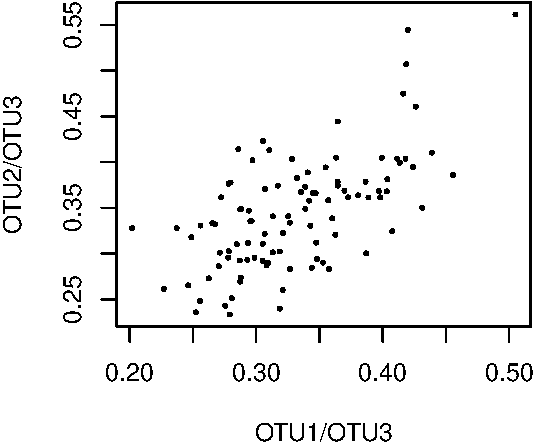
\includegraphics{main_files/figure-latex/R_block_correlation-1.pdf}
\caption{\label{correlation} Spurious correlation in compositional data.
Two random vectors drawn from a Normal distribution, were divided by a
third vector also drawn at random from a Normal distribution. The two
vectors have nothing in common, they should exhibit no correlation, and
yet they exhibit a correlation coefficent of \(>0.65\) when divided by
the third vector. See the introductory section of the Supplementary
Information of Lovell (2015) for a more complete description of this
phenomenon.}
\end{figure}

\subsubsection{Sub-compositions}\label{sub-compositions}

Compositional data have the third property of a sub-composition
incoherence of correlation metrics. That is,
\emph{correlations calculated on compositional datasets are unique to the particular dataset chosen}
(Aitchison, 1986). This is problematic because high throughput
sequencing experimental designs are \emph{always} sub-compositions.
Inspection of papers in the literature provide many examples. For
example, in the 16S rRNA gene sequencing literature it is common
practice to discard rare OTU species prior to analysis and to
re-normalize by dividing the counts for the remaining OTUs by the new
sample sum. It is also common to use only one or a few taxonomic
groupings to determine differences between experimental conditions. In
the case of RNA-seq only the fraction of RNA of interest is sequenced,
usually mRNA but other sub-fractions such as miRNA may be sequenced. All
of these practices expose the investigator to the problem of
non-coherence between sub-compositions. We must use
compositionally-appropriate measures of correlation---more formally, we
are attempting to find features that are compositionally associated.
Compositional association is a more restricted measure of correlation
and is explained more completely in the chapter on data transformations.

To summarize, compositional data has the following pathologies:

\begin{itemize}
\item
  The negative correlation bias means that any negative correlation
  observed in compositional data must be treated as suspect because it
  could arise simply because a different feature (or features) changed
  their abundance. There is currently no theoretically valid approach to
  identify true negative correlations in compositional data (Egozcue et
  al., 2018).
\item
  The spurious correlation problem means that we can observe apparent
  postive correlations simply by chance. I describe recent work that
  shows that spurious correlation is tractable.
\item
  The sub-compositional incoherence of correlation is perhaps the most
  insidious property, but also the easiest to recognize. Here the
  correlation depends on the \emph{exact} set of features present in the
  dataset. If the observed correlations change when the data are subset,
  then sub-compositional incoherence is in play.
\end{itemize}

Thus, one major reason to use compositional data methods is that you are
more likely to report robust results, and the later practical chapters
demonstrate the robustness of a compositional data analysis.

Practically speaking the negative correlation bias, the occurrence of
spurious correlation, and the problem of sub-compositional incoherence
means that
\emph{every microbial correlation network that has ever been published is suspect},
as is \emph{every gene co-occurrence or co-expression network} unless
compositionally appropriate compositional association metric was used
(Erb and Notredame, 2016; Lovell et al., 2015; Quinn et al., 2017a).
These approaches themselves have limitations and as originally
constituted cannot deal with sparse data. However, recasting the data
from count compositions to probability distributions allows these
methods to be adapted to sparse data with some success (Bian et al.;
Quinn et al., 2017a).

\subsection{So can I analyze compositional data?
How?}\label{so-can-i-analyze-compositional-data-how}

Much of the high throughput sequencing analysis literature seems to
assume that data derived from high throughput sequencing are in some way
unique, and that purpose-built tools must be used. However, there is
nothing special about high-throughput sequencing data from the point of
view of the analysis. Fortunately, the analysis of compositional
datasets has a well-developed methodology (Pawlowsky-Glahn et al., 2015;
Van den Boogaart and Tolosana-Delgado, 2013), much of which was worked
out in the geological sciences.

Atichison (1986), Pawlsky-Glahn (2006), and Egozcue (2005), have done
much work to develop rigorous approaches to analyze compositional data
(Pawlowsky-Glahn and Buccianti, 2011). The essential step is to reduce
the data to ratios between the \(D\). This step does not move the data
from the Simplex but does transform the data on the Simplex such that
the distances between the ratios of the features are linear. The
investigator must keep in mind that the distances are between ratios
between features, not between counts of features (re-read this several
times to wrap your head around it). Several transformations are in
common use, but the one I believe is most applicable to HTS data is the
centred log-ratio transformation or clr, where the data in each sample
is transformed by taking the logarithm of the the ratio between the
count value for each part and the geometric mean count: i.e., for D
features in sample vector \(\vect{X} = [x_1, x_2, x_3, \ldots x_D]\):

\begin{equation}
 \vect{X}_{clr}  = [log(\frac{x_1}{gX}), log(\frac{x_2}{gX}) \ldots log(\frac{x_D}{gX})]
\end{equation}

where \(gX\) is the geometric mean of the features in sample
\(\vect{X}\). The clr transformation is formally equivalent to a matrix
of all possible pairwise ratios, but is a more tractable form. The clr
transformation is not perfect by any means, but when there are large
numbers of features the properties of the clr approach the ideal
isometric log-ratio transformation or ilr. In the context of high
throughput sequencing, where there are often hundreds or thousands of
features the clr and the ilr have nearly indistinguishable properties.

The properties of the clr transformation are demonstrated in the chapter
on data transformations.

\clearpage

\section{Data transforms in high throughput
sequencing}\label{data-transforms-in-high-throughput-sequencing}

This chapter introduces data transformations that are prevalent in the
ecological literature, and that have been extensively used in analyzing
high throughput sequencing datasets. It is not intended to be a
comprehensive analysis of data transformations, nor are all
transformations described. In some cases, only one transformation is
demonstrated when several transformations are obviously related. The
\texttt{vegan} R package manual (Oksanen et al., 2017) has a very good
description of many other data transformations and I recommend it to the
interested reader: note that the \texttt{vegan} package is not
compositionally appropriate.

This chapter is rather information dense, but the lessons in it are very
important to understand the limitations of data analysis whenever the
data are compositional. I have tried to make it easy and intuitive, but
in the end you must work through the examples as best you can. All the
source code needed to explore the data are included either directly
here, or in an external file when the amount of code would break the
flow of the narrative.

It is assumed that the output from a high-throughput sequencing
experiment represents in some way the underlying abundance of the input
DNA molecules. The input counts panels on the left side of Figure
\ref{fig_shape} shows two idealized experiments. The top left shows the
case where the total count of all nucleic acid species in the input is
constrained, the bottom left illustrates the case where the total count
is unconstrained. These are modelled as a time series, but any process
would produce the same results.

Constrained datasets occur if the increase or decrease in any component
is exactly compensated by the increase or decrease of one or more
others. Here the total count remains constant across all experimental
conditions. Examples of constrained datasets would include allele
frequencies at a locus where the total has to be 1, and the RNA-seq
where the induction of genes occurs in a steady-state cell culture. In
this case, any process, such as sequencing that generates a proportion
simply recapitulates the data with sampling error. The unspoken
assumption in most high throughput experimental designs is that this
assumption is true---\emph{ it is not!}

An unconstrained dataset results if the total count is free to vary.
Examples of unconstrained datasets would include ChIP-Seq, RNA-seq where
we are examining two different conditions or cell populations,
metagenomics, etc. Importantly, 16S rRNA gene sequencing analyses are
almost always free to vary; that is, the total bacterial load is rarely
constant in an environment. Thus, the unconstrained data type would be
the predominant type of data that would be expected.

The relative abundance panels on the right side of Figure
\ref{fig_shape} shows the result of random sampling with a defined
maximum value in these two types of datasets. This random sampling
reflects the data that results from high throughput sequencing where the
total number of reads is constrained by the instrument capacity. The
data is represented as a proportion, but scales to parts per million or
parts per billion without changing the shape. Here we see that the shape
of the data after sequencing is very similar to the input data in the
case of constrained, but is very different in the case of
non-constrained data. In the unconstrained dataset, observe how the blue
and red features appear to be constant over the first 10 time points,
but then appear to decrease in abundance at later time points.
Conversely, the black feature appears to increase linearly at early time
points, but appears to become constant at late time points. Obviously,
we would misinterpret what is happening if we compared early and late
timepoints in the unconstrained dataset. It is also worth noting how the
act of random sampling makes the proportional abundance of the rare OTU
species uncertain in both the constrained and unconstrained data, but
has little effect on the relative apparent effect on the relative
abundance of OTUs with high counts.

\subsection{Sequencing can change the shape of the
data:}\label{sequencing-can-change-the-shape-of-the-data}

\begin{Shaded}
\begin{Highlighting}[]
\CommentTok{# the number of rare counts in the dataset}
\NormalTok{num.one =}\StringTok{ }\DecValTok{100}
\NormalTok{ncol=num.one +}\StringTok{ }\DecValTok{10}

\NormalTok{m.dub <-}\StringTok{ }\KeywordTok{matrix}\NormalTok{(}\DataTypeTok{data=}\OtherTok{NA}\NormalTok{, }\DataTypeTok{nrow=}\DecValTok{20}\NormalTok{, }\DataTypeTok{ncol=}\NormalTok{ncol)}
\NormalTok{prop.m <-}\StringTok{ }\KeywordTok{matrix}\NormalTok{(}\DataTypeTok{data=}\OtherTok{NA}\NormalTok{, }\DataTypeTok{nrow=}\DecValTok{20}\NormalTok{, }\DataTypeTok{ncol=}\NormalTok{ncol)}
\NormalTok{clr.m <-}\StringTok{ }\KeywordTok{matrix}\NormalTok{(}\DataTypeTok{data=}\OtherTok{NA}\NormalTok{, }\DataTypeTok{nrow=}\DecValTok{20}\NormalTok{, }\DataTypeTok{ncol=}\NormalTok{ncol)}

\NormalTok{m.dub.u <-}\StringTok{ }\KeywordTok{matrix}\NormalTok{(}\DataTypeTok{data=}\OtherTok{NA}\NormalTok{, }\DataTypeTok{nrow=}\DecValTok{20}\NormalTok{, }\DataTypeTok{ncol=}\NormalTok{ncol)}
\NormalTok{prop.m.u <-}\StringTok{ }\KeywordTok{matrix}\NormalTok{(}\DataTypeTok{data=}\OtherTok{NA}\NormalTok{, }\DataTypeTok{nrow=}\DecValTok{20}\NormalTok{, }\DataTypeTok{ncol=}\NormalTok{ncol)}
\NormalTok{clr.m.u <-}\StringTok{ }\KeywordTok{matrix}\NormalTok{(}\DataTypeTok{data=}\OtherTok{NA}\NormalTok{, }\DataTypeTok{nrow=}\DecValTok{20}\NormalTok{, }\DataTypeTok{ncol=}\NormalTok{ncol)}

\NormalTok{in.put <-}\StringTok{ }\KeywordTok{c}\NormalTok{(}\DecValTok{10}\NormalTok{,}\DecValTok{20971}\NormalTok{,}\DecValTok{1}\NormalTok{,}\DecValTok{1}\NormalTok{,}\DecValTok{5}\NormalTok{,}\DecValTok{10}\NormalTok{,}\DecValTok{20}\NormalTok{,}\DecValTok{50}\NormalTok{,}\DecValTok{100}\NormalTok{,}\DecValTok{200}\NormalTok{,}\DecValTok{1000}\NormalTok{)}

\NormalTok{total.sum <-}\StringTok{ }\KeywordTok{sum}\NormalTok{(in.put +}\StringTok{ }\DecValTok{1}\NormalTok{) *}\StringTok{ }\DecValTok{1000}

\CommentTok{# constrained with Gaussian noise}
\CommentTok{# one feature increases exponentially}
\CommentTok{# one feature decreases to compensate}
\NormalTok{for(i in }\DecValTok{0}\NormalTok{:}\DecValTok{19}\NormalTok{)\{}
    \NormalTok{junk <-}\StringTok{ }\NormalTok{in.put *}\StringTok{ }\KeywordTok{c}\NormalTok{(}\DecValTok{2}\NormalTok{^i,}
        \KeywordTok{rep}\NormalTok{(}\DecValTok{1}\NormalTok{,num.one +}\StringTok{ }\DecValTok{9}\NormalTok{))}
    \NormalTok{junk[}\DecValTok{3}\NormalTok{] <-}\StringTok{ }\NormalTok{total.sum -}\StringTok{ }\KeywordTok{sum}\NormalTok{(junk)}
    \NormalTok{m.dub[i}\DecValTok{+1}\NormalTok{,] <-}\StringTok{ }\NormalTok{junk}
    \NormalTok{prop.m[i}\DecValTok{+1}\NormalTok{,] <-}\StringTok{ }\KeywordTok{as.numeric}\NormalTok{(}
        \KeywordTok{rdirichlet}\NormalTok{(}\DecValTok{1}\NormalTok{, junk) )}
    \NormalTok{clr.m[i}\DecValTok{+1}\NormalTok{,] <-}\StringTok{ }\KeywordTok{log2}\NormalTok{(prop.m[i}\DecValTok{+1}\NormalTok{,])}
        \NormalTok{-}\StringTok{ }\KeywordTok{mean}\NormalTok{(}\KeywordTok{log2}\NormalTok{(prop.m[i}\DecValTok{+1}\NormalTok{,]))}
\NormalTok{\}}
\CommentTok{# non-constrained with Gaussian noise}
\CommentTok{# same as above, without the decreasing}
\CommentTok{# feature}
\NormalTok{for(i in }\DecValTok{0}\NormalTok{:}\DecValTok{19}\NormalTok{)\{}
    \NormalTok{junk <-}\StringTok{ }\NormalTok{in.put *}\StringTok{ }\KeywordTok{c}\NormalTok{(}\DecValTok{2}\NormalTok{^i,}
        \KeywordTok{rep}\NormalTok{(}\DecValTok{1}\NormalTok{,num.one +}\StringTok{ }\DecValTok{9}\NormalTok{))}
    \NormalTok{m.dub.u[i}\DecValTok{+1}\NormalTok{,] <-}\StringTok{ }\NormalTok{junk}
    \NormalTok{prop.m.u[i}\DecValTok{+1}\NormalTok{,] <-}\StringTok{ }\KeywordTok{as.numeric}\NormalTok{(}
        \KeywordTok{rdirichlet}\NormalTok{(}\DecValTok{1}\NormalTok{, junk) )}
    \NormalTok{clr.m.u[i}\DecValTok{+1}\NormalTok{,] <-}\StringTok{ }\DecValTok{2}\NormalTok{^(}\KeywordTok{log2}\NormalTok{(prop.m.u[i}\DecValTok{+1}\NormalTok{,])}
        \NormalTok{-}\StringTok{ }\KeywordTok{mean}\NormalTok{(}\KeywordTok{log2}\NormalTok{(prop.m.u[i}\DecValTok{+1}\NormalTok{,])))}
\NormalTok{\}}

\NormalTok{plot_c <-}\StringTok{ }\NormalTok{function(x, main, ylab, }\DataTypeTok{log=}\StringTok{""}\NormalTok{)\{}
    \KeywordTok{plot}\NormalTok{(x[,}\DecValTok{1}\NormalTok{], }\DataTypeTok{pch=}\DecValTok{20}\NormalTok{, }\DataTypeTok{type=}\StringTok{"b"}\NormalTok{,  }\DataTypeTok{log=}\NormalTok{log,}
    \DataTypeTok{ylim=}\KeywordTok{c}\NormalTok{(}\KeywordTok{min}\NormalTok{(x), }\KeywordTok{max}\NormalTok{(x)), }\DataTypeTok{xlab=}\StringTok{"time point"}\NormalTok{,}
    \DataTypeTok{ylab=}\NormalTok{ylab)}
    \KeywordTok{title}\NormalTok{( }\DataTypeTok{main=}\NormalTok{main, }\DataTypeTok{adj=}\FloatTok{0.5}\NormalTok{)}
    \KeywordTok{points}\NormalTok{(x[,}\DecValTok{2}\NormalTok{], }\DataTypeTok{type=}\StringTok{"b"}\NormalTok{,}\DataTypeTok{pch=}\DecValTok{21}\NormalTok{, }\DataTypeTok{col=}\StringTok{"gray"}\NormalTok{)}
    \KeywordTok{points}\NormalTok{(x[,}\DecValTok{3}\NormalTok{], }\DataTypeTok{type=}\StringTok{"b"}\NormalTok{,}\DataTypeTok{pch=}\DecValTok{22}\NormalTok{, }\DataTypeTok{col=}\StringTok{"orange"}\NormalTok{)}
    \KeywordTok{points}\NormalTok{(x[,num.one +}\StringTok{ }\DecValTok{10}\NormalTok{], }\DataTypeTok{type=}\StringTok{"b"}\NormalTok{,}
        \DataTypeTok{pch=}\DecValTok{23}\NormalTok{, }\DataTypeTok{col=}\StringTok{"blue"}\NormalTok{)}
    \KeywordTok{points}\NormalTok{(x[,num.one}\DecValTok{+4}\NormalTok{], }\DataTypeTok{type=}\StringTok{"b"}\NormalTok{, }\DataTypeTok{pch=}\DecValTok{24}\NormalTok{,}
        \DataTypeTok{col=}\StringTok{"red"}\NormalTok{)}
\NormalTok{\}}

\KeywordTok{par}\NormalTok{(}\DataTypeTok{mfrow=}\KeywordTok{c}\NormalTok{(}\DecValTok{2}\NormalTok{,}\DecValTok{4}\NormalTok{), }\DataTypeTok{mar=}\KeywordTok{c}\NormalTok{(}\DecValTok{4}\NormalTok{,}\DecValTok{4}\NormalTok{,}\DecValTok{3}\NormalTok{,}\DecValTok{1}\NormalTok{) )}

\CommentTok{#constrained}
\KeywordTok{plot_c}\NormalTok{(m.dub, }\DataTypeTok{main=}\StringTok{"Constrained}\CharTok{\textbackslash{}n}\StringTok{count"}\NormalTok{,}
    \DataTypeTok{ylab=}\StringTok{"raw count"}\NormalTok{)}
\KeywordTok{plot_c}\NormalTok{(prop.m, }\DataTypeTok{main=}\StringTok{"Constrained}\CharTok{\textbackslash{}n}\StringTok{proportion"}\NormalTok{,}
    \DataTypeTok{ylab=}\StringTok{"raw proportion"}\NormalTok{)}
\KeywordTok{plot_c}\NormalTok{(m.dub, }\DataTypeTok{main=}\StringTok{"Constrained}\CharTok{\textbackslash{}n}\StringTok{count"}\NormalTok{,}
    \DataTypeTok{ylab=}\StringTok{"log10 count"}\NormalTok{, }\DataTypeTok{log=}\StringTok{"y"}\NormalTok{)}
\KeywordTok{plot_c}\NormalTok{(prop.m, }\DataTypeTok{main=}\StringTok{"Constrained}\CharTok{\textbackslash{}n}\StringTok{proportion"}\NormalTok{,}
    \DataTypeTok{ylab=}\StringTok{"log10 proportion"}\NormalTok{, }\DataTypeTok{log=}\StringTok{"y"}\NormalTok{)}

\CommentTok{# unconstrained}
\KeywordTok{plot_c}\NormalTok{(m.dub.u, }\DataTypeTok{main=}\StringTok{"Unconstrained}\CharTok{\textbackslash{}n}\StringTok{count"}\NormalTok{,}
    \DataTypeTok{ylab=}\StringTok{"raw count"}\NormalTok{)}
\KeywordTok{plot_c}\NormalTok{(prop.m.u, }\DataTypeTok{main=}\StringTok{"Unconstrained}\CharTok{\textbackslash{}n}\StringTok{proportion"}\NormalTok{,}
    \DataTypeTok{ylab=}\StringTok{"raw proportion"}\NormalTok{)}
\KeywordTok{plot_c}\NormalTok{(m.dub.u, }\DataTypeTok{main=}\StringTok{"Unconstrained}\CharTok{\textbackslash{}n}\StringTok{count"}\NormalTok{,}
     \DataTypeTok{ylab=}\StringTok{"log10 count"}\NormalTok{, }\DataTypeTok{log=}\StringTok{"y"}\NormalTok{)}
\KeywordTok{plot_c}\NormalTok{(prop.m.u, }\DataTypeTok{main=}\StringTok{"Unconstrained}\CharTok{\textbackslash{}n}\StringTok{proportion"}\NormalTok{,}
     \DataTypeTok{ylab=}\StringTok{"log10 proportion"}\NormalTok{, }\DataTypeTok{log=}\StringTok{"y"}\NormalTok{)}
\end{Highlighting}
\end{Shaded}

\begin{figure}[htbp]
\centering
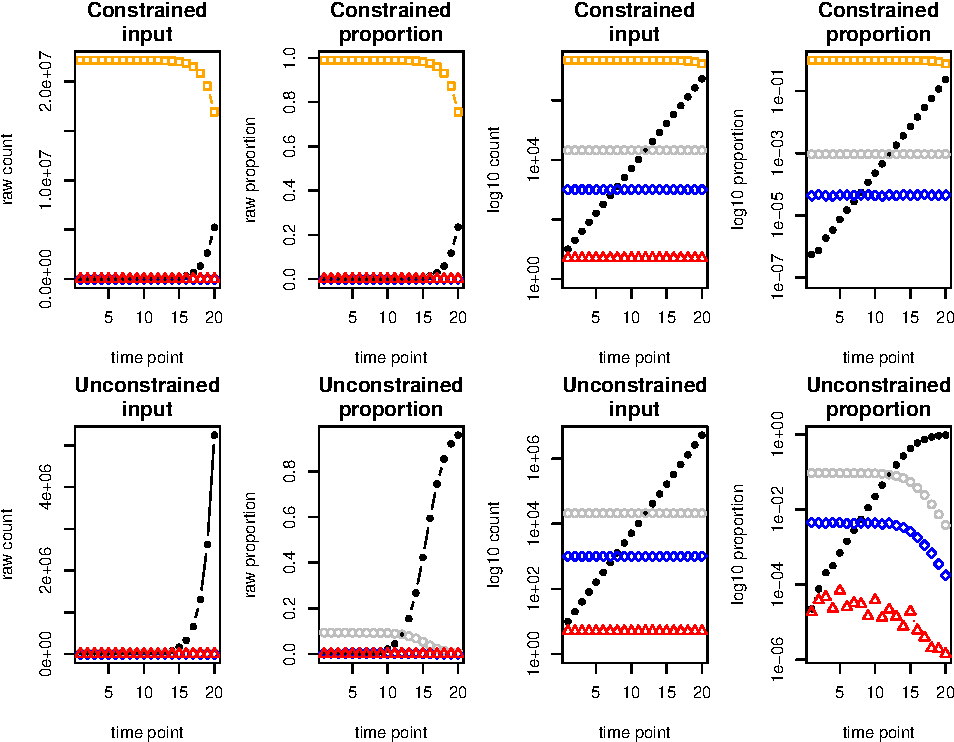
\includegraphics{main_files/figure-latex/R_block_constrained_data-1.pdf}
\caption{\label=\{fig-shape\}High-throughput sequencing affects the
shape of the data differently on constrained and unconstrained data. The
two left panels show the absolute number of reads in the input tube for
20 steps where the green and black OTUs are changing abundance by 2-fold
each step. The gray, blue and red OTUs are held at a constant number in
each step in both cases. The second column shows the output in
proportions (or ppm, or FPKM) after random sampling to a constant sum,
as occurs on the sequencer. The orange OTU in the constrained data set
is much more abundant than any other, and is changing to maintain a
constant number of input molecules. Samples in the two right columns are
the same values plotted on a log scale on the Y-axis for convenience.
Note how the constrained data is the same before and after sequencing
while the unconstrained data is severely distorted.}
\end{figure}

We assume that the abundance of each input DNA species that is observed
after sequencing reflects a random sample of the input molecules. We can
see that that this may indeed be the case if the total number of
molecules in the input sample is constant. This constraint would be met
if, for example, an increase in one or more DNA species was balanced
with an equivalent decrease in one or more different species. Such a
constraint would be met In the figure, the red and blue OTU sequences
are held constant in each sample, the green OTU is decreasing by 2 fold
and the black OTU is increasing by 2 fold in each subsequent sample. The
abundance of the orange OTU is adjusted such that the total sum of the
OTU sequences in the input is held constant. Here it can be seen that
the input counts and the relative abundance of each species following
sequence have similar shapes, with the exception that the rarest species
display significant variability because of random sampling.

\subsection{Commonly used transformations are
misleading}\label{commonly-used-transformations-are-misleading}

Current practice is to examine the datasets using `relative abundance'
values, that is, the proportional abundance of the OTUs either before or
after normalization for read depth. This approach is equivalent to
examining the input unconstrained data of the type seen in Figure
\ref{fig_shape} in the relative abundance sample space in the bottom
right panel of the figure. This approach will obviously lead to
incorrect assumptions in at least some cases. For example, depending
upon the steps chosen to compare, the blue OTU, that has constant counts
in the input, will be seen to either increase or decrease in abundance.
Conversely, the green OTU, that is always decreasing in abundance will
be seen to be constant if comparing samples 1-8.

The ecological literature offers many different transformations for such
data, often as a way of making the data appear `more normal'. Figure
\ref{transform} shows the results of five such transformations.

\begin{itemize}
\item
  The frequency transform divides the each OTU value by the largest OTU
  count, and then divides the resulting values by the number of OTUs in
  the sample that had non-zero counts.
\item
  The Hellinger transformation that takes the square root of the
  relative abundance (proportion) value.
\item
  The range transform standardizes the values to have a range from 0 to
  1. OTUs with 0 counts are set to 0.
\item
  The standardize transform standardizes the values for each sample to
  have a mean of 0 and a variance of 1.
\item
  The log transform divides each OTU count in a sample by the minimum
  non-zero count value, then takes the logarithm of the resulting value
  and adds 1. Counts of 0 are assigned a value of 0 to avoid taking the
  logarithm of 0.
\item
  The centred log-ratio transformation divides the OTU values by the
  geometric mean OTU abundance, and then takes the logarithm.
\end{itemize}

It is obvious that the first four transformations result in data that
badly mis-represents the shape of the actual input data. The log
transformation, however results in the shape of the output data
approximating the shape of the input data, except that the uncertainty
of each data point is large. The ratio transform his transformation
accurately recapitulates the shape of the original input data, and more
accurately represents the uncertainty of each data point.

\begin{figure}[htbp]
\centering
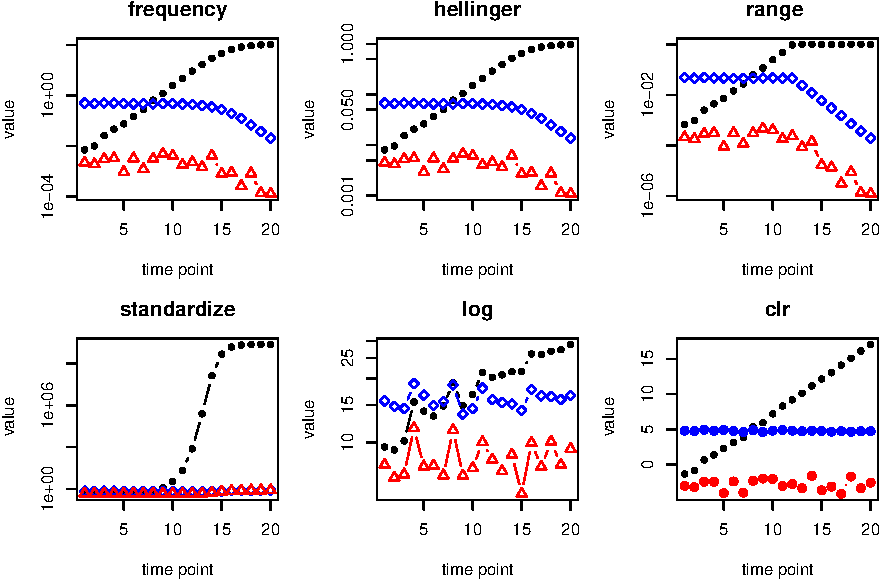
\includegraphics{main_files/figure-latex/R_block_transformations-1.pdf}
\caption{\label{transforms} The effect of ecological transformations on
unconstrained high throughput sequencing datasets. Data generated as in
Figure \ref{fig_shape} were transformed with five different approaches
implemented in the vegan ecological analysis package, and with the
entered log-ratio approach suggested by Aitchison.}
\end{figure}

Fundamentally, the goal of any experiment is to determine something
about the environment that was sampled. After all, we are attempting to
use HTS to determine something of interest about the underlying
environment. Thus, we need to have some equivalence between the samples
before sequencing and the samples after sequencing. The simplest case
would be that there would be a linear relationship between the data that
we could obtain from the environment, and the data that was actually
collected by HTS.

We can think about the underlying data on a univariate basis; do the
features across all samples follow a Gaussian distribution? or do they
follow some unknown distribution? If so, can we transform the data to
approximate a Gaussian distribution? This mode of thinking leads to the
use of square-root, arcsine or Hellinger transformations since they
appear to transform the data into a distribution that can be
interpreted. However, as we shall see below, none of these univariate
transformations is suitable.

It is more desirable to think about HTS data in a multivariate way as a
`composition' because the total count of molecules in the underlying
sample (the environment) is always a confounding variable (Lovén et al.,
2012). This way of thinking led to multivariate data normalizations.

We will set up a random dataset, composed of four features (T, L, G, A)
and 50 random samples with mean values of 100 tigers, 10000 ladybugs,
1000 gnus and 5 space aliens. The features will be drawn from a Normal
distibution, although a random uniform distribution or any other
distribution will give the same results. We are not, at this point,
attempting to mimic a distribution found in a real dataset, but are
instead showing the general properties of the distance metrics, and how
those metrics compare when calculated on numerical data, obtained as
counts in the environment, or on proportional data, obtained as relative
abundances after sequencing.

\begin{Shaded}
\begin{Highlighting}[]
\KeywordTok{set.seed}\NormalTok{(}\DecValTok{13}\NormalTok{)}
\NormalTok{T <-}\StringTok{ }\KeywordTok{rnorm}\NormalTok{(}\DecValTok{50}\NormalTok{, }\DataTypeTok{mean=}\DecValTok{100}\NormalTok{, }\DataTypeTok{sd=}\DecValTok{25}\NormalTok{)}
\NormalTok{L <-}\StringTok{ }\KeywordTok{rnorm}\NormalTok{(}\DecValTok{50}\NormalTok{, }\DataTypeTok{mean=}\DecValTok{10000}\NormalTok{, }\DataTypeTok{sd=}\DecValTok{2500}\NormalTok{)}
\NormalTok{G <-}\StringTok{ }\KeywordTok{rnorm}\NormalTok{(}\DecValTok{50}\NormalTok{, }\DataTypeTok{mean=}\DecValTok{1000}\NormalTok{, }\DataTypeTok{sd=}\DecValTok{250}\NormalTok{)}
\NormalTok{A <-}\StringTok{ }\KeywordTok{rnorm}\NormalTok{(}\DecValTok{50}\NormalTok{, }\DataTypeTok{mean=}\DecValTok{5}\NormalTok{, }\DataTypeTok{sd=}\FloatTok{2.5}\NormalTok{)}
\NormalTok{ran.dat <-}\StringTok{ }\KeywordTok{cbind}\NormalTok{(T,L,G,A)}
\NormalTok{ran.dat[ran.dat <=}\DecValTok{0} \NormalTok{] <-}\StringTok{ }\FloatTok{0.1}

\NormalTok{dist.ran.dat <-}\StringTok{ }\KeywordTok{as.matrix}\NormalTok{(}\KeywordTok{dist}\NormalTok{(}
    \NormalTok{ran.dat, }\DataTypeTok{method=}\StringTok{"euclidian"}\NormalTok{))}

\KeywordTok{par}\NormalTok{(}\DataTypeTok{mfrow=}\KeywordTok{c}\NormalTok{(}\DecValTok{1}\NormalTok{,}\DecValTok{3}\NormalTok{), }\DataTypeTok{pch=}\DecValTok{19}\NormalTok{, }\DataTypeTok{col=}\KeywordTok{rgb}\NormalTok{(}\DecValTok{0}\NormalTok{,}\DecValTok{0}\NormalTok{,}\DecValTok{0}\NormalTok{,}\FloatTok{0.5}\NormalTok{),}
    \DataTypeTok{cex=}\FloatTok{1.5}\NormalTok{, }\DataTypeTok{cex.lab=}\FloatTok{1.5}\NormalTok{)}

\KeywordTok{plot}\NormalTok{(T,L)}
\KeywordTok{plot}\NormalTok{(L,G)}
\KeywordTok{plot}\NormalTok{(G,A)}
\end{Highlighting}
\end{Shaded}

\begin{figure}[htbp]
\centering
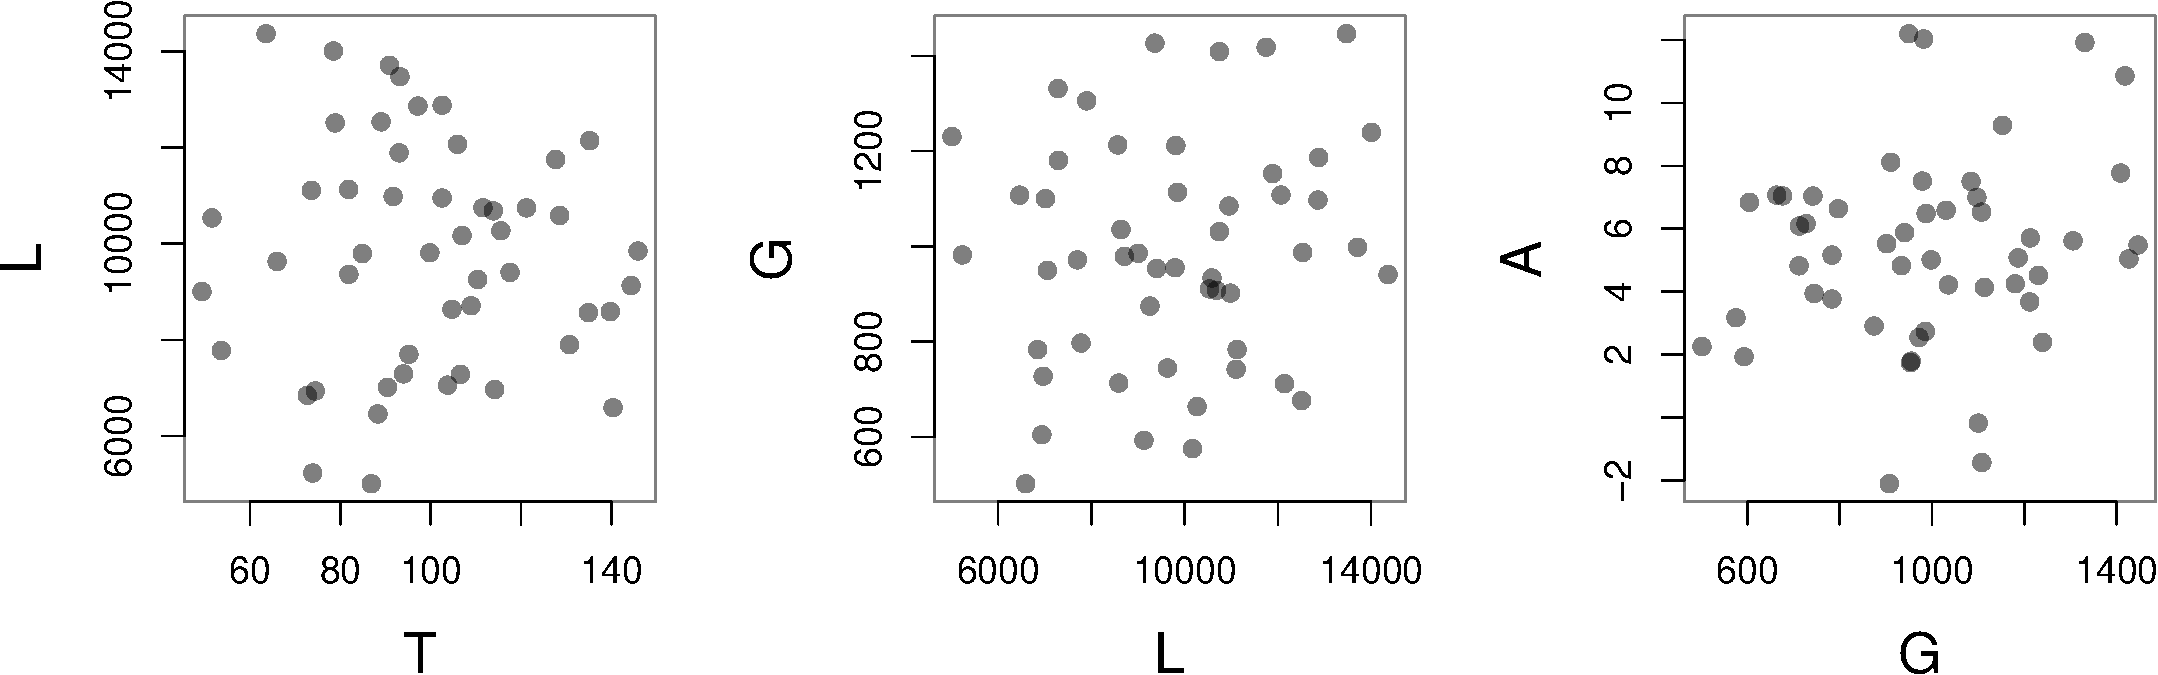
\includegraphics{main_files/figure-latex/R_block_random-1.pdf}
\caption{\label{numbers} Plot of Ladybugs vs.~Tigers, Gnus vs.~Ladybugs
and Aliens vs.~Gnus for simulated random Normal data.}
\end{figure}

Figure \ref{numbers} shows the relationships between three features in
the actual dataset. We can see that the features are randomly normally
distributed and uncorrelated in the scatter plots. Most tools attempt to
infer something about this numerical dataset. For this to work, the data
transforms must be linearly related in some way to this underlying data.

Let us see which, if any of the transforms fulfills this basic
requirement.

\subsection{Notation}\label{notation}

We use the following notation throughout. Column vectors contain samples
\(\vec{\textbf{s}}\) and row vectors contain features
\(\vec{\textbf{f}}\). There are \(D\) features and \(n\) samples, thus
the data are contained in matrix \(M = D \times n\). The \(j^{th}\)
sample is denoted as \(s_{j}\), the \(i^{th}\) feature of all samples is
denoted as \(s_{i-}\), and the value for the \(i^{th}\) feature of the
\(j^{th}\) sample is referred to as \(s_{ij}\).

\subsection{Simple proportional type
transformations}\label{simple-proportional-type-transformations}

The simplest normalization is to determine the relative abundance (rAB),
or proportion, of the \ith{i} feature in a sample as in Eq.
\ref{eq:rab}. This normalization is also referred to as the total sum
scaling (TSS) normalization.

\begin{equation}
    rAB_{i} = \frac{s_{i}}{\sum{\vec{\textbf{s}}}}
    \label{eq:rab}
\end{equation}

The rAB measure requires only the read count observed for a the feature
\(s_i\) and the total read count of the sample
\(\sum{\vec{\textbf{s}}}\). Since this measure is generally skewed, it
is often log-transformed prior to analysis.

\begin{Shaded}
\begin{Highlighting}[]
\NormalTok{ran.dat.prop <-}\StringTok{ }\KeywordTok{t}\NormalTok{(}\KeywordTok{apply}\NormalTok{(ran.dat, }\DecValTok{1}\NormalTok{,}
    \NormalTok{function(x) x/}\KeywordTok{sum}\NormalTok{(x)))}
\KeywordTok{par}\NormalTok{(}\DataTypeTok{mfrow=}\KeywordTok{c}\NormalTok{(}\DecValTok{1}\NormalTok{,}\DecValTok{3}\NormalTok{), }\DataTypeTok{pch=}\DecValTok{19}\NormalTok{, }\DataTypeTok{col=}\KeywordTok{rgb}\NormalTok{(}\DecValTok{0}\NormalTok{,}\DecValTok{0}\NormalTok{,}\DecValTok{0}\NormalTok{,}\FloatTok{0.5}\NormalTok{),}
    \DataTypeTok{cex=}\FloatTok{1.5}\NormalTok{, }\DataTypeTok{cex.lab=}\FloatTok{1.5}\NormalTok{)}
\KeywordTok{plot}\NormalTok{(ran.dat.prop[,}\StringTok{"T"}\NormalTok{],ran.dat.prop[,}\StringTok{"L"}\NormalTok{],}
    \DataTypeTok{xlab=}\StringTok{"T.p"}\NormalTok{, }\DataTypeTok{ylab=}\StringTok{"L.p"}\NormalTok{)}
\KeywordTok{plot}\NormalTok{(ran.dat.prop[,}\StringTok{"L"}\NormalTok{],ran.dat.prop[,}\StringTok{"G"}\NormalTok{],}
    \DataTypeTok{xlab=}\StringTok{"L.p"}\NormalTok{, }\DataTypeTok{ylab=}\StringTok{"G.p"}\NormalTok{)}
\KeywordTok{plot}\NormalTok{(ran.dat.prop[,}\StringTok{"G"}\NormalTok{],ran.dat.prop[,}\StringTok{"A"}\NormalTok{],}
    \DataTypeTok{xlab=}\StringTok{"G.p"}\NormalTok{, }\DataTypeTok{ylab=}\StringTok{"A.p"}\NormalTok{)}
\end{Highlighting}
\end{Shaded}

\begin{figure}[htbp]
\centering
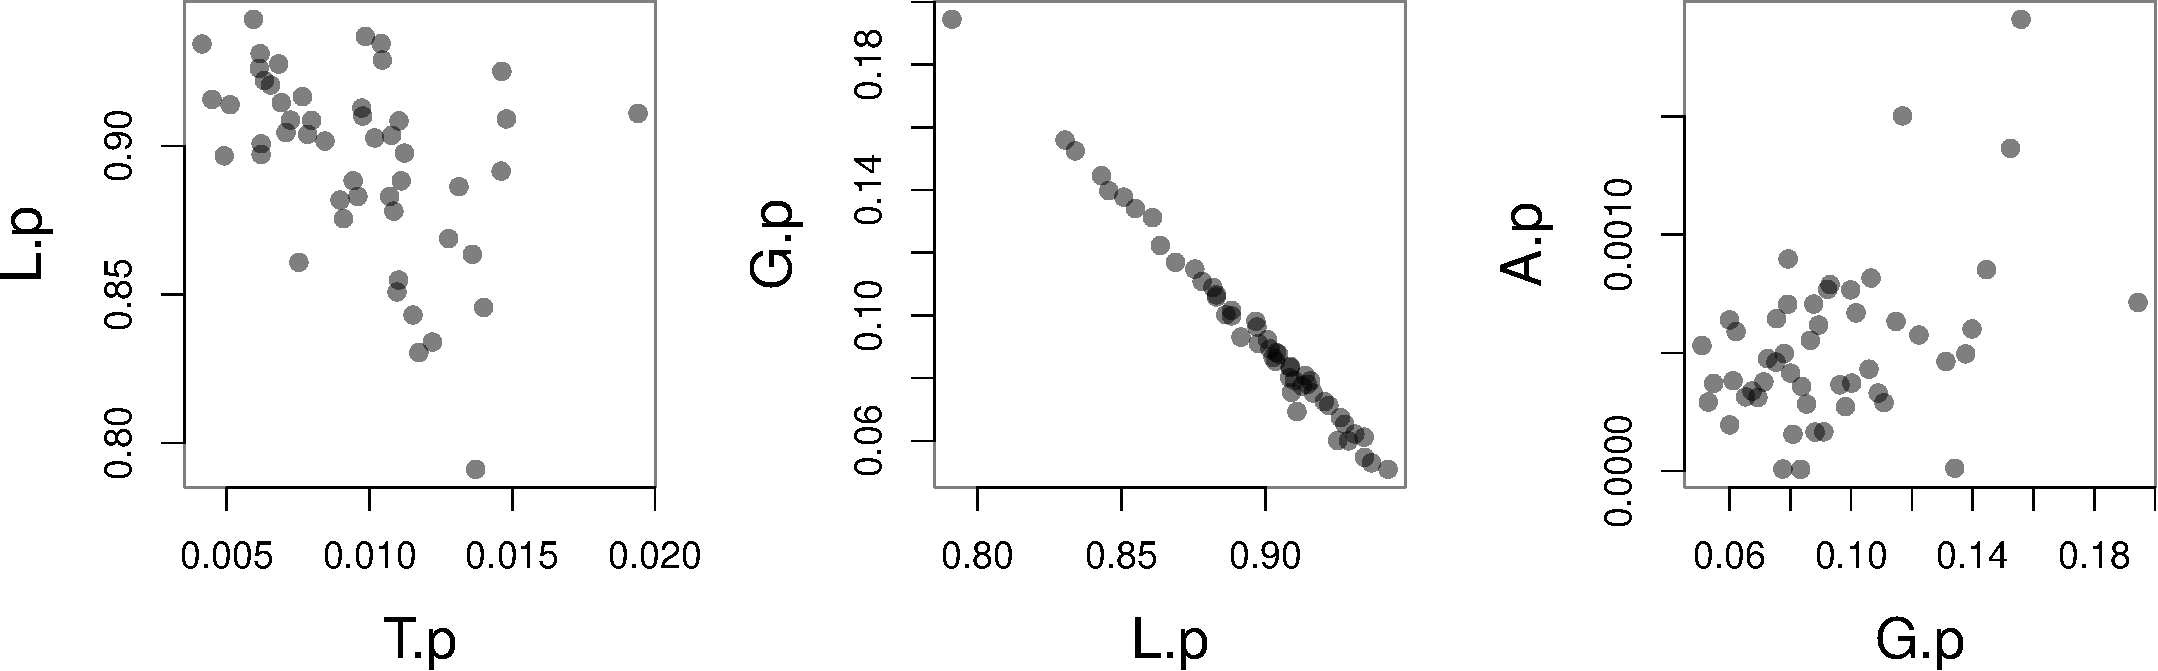
\includegraphics{main_files/figure-latex/R_block_TSS-1.pdf}
\caption{\label{numbers} Plot of Ladybugs vs.~Tigers, Gnus vs.~Ladybugs
and Aliens vs.~Gnus for simulated random Normal data as proportions.}
\end{figure}

By comparing the proportions to the non-transformed data, we can see
that the structure of the data itself has changed dramatically. The two
most abundant features, G and L, which are uncorrelated in the actual
data are now almost perfectly negatively correlated when the same data
are converted and plotted as proportions, G.p vs L.p.~This is because
the data are now not real numbers, but are instead proportions and are
constrained by the arbitrary sum of 1:
\emph{the data are now compositional data}.

A further normalization was proposed early in the RNA-seq field where
the reads per kilobase per million mapped (RPKM)(Mortazavi et al., 2008)
method was used initially to place the read counts for each feature
within and between samples on a common scale.

For this we also needed to know a scaling factor \(K\), and the length
of the feature \(L_i\); from this, the RPKM value for the \ith{i}
feature for each sample was calculated as in Eq. \ref{eq:rpkm}.

\begin{equation}
    RPKM_{i} = \frac{K \cdot C_{i} }{\sum{C} \cdot L_{i}}
    \label{eq:rpkm}
\end{equation}

When the equation is placed in this form it is obvious that RPKM is
simply a scaled rAB where each rAB value is divided by its length and
multiplied by a constant. In compositional terms, RPKM is an unclosed
perturbation of the original data; the data appear to be real numbers,
but are actually proportions multiplied by a constant.

Further research suggested that RPKM was not appropriate for comparison
of features between samples. The goal of RPKM was to `count' reads per
feature per cell. In the original paper the authors supplied an
equivalence and an RPKM value of 1 RPKM equalled one transcript in each
cell in the C2C12 cell line, but in liver cells, a value of 3 RPKM
equalled one transcript per cell. Thus, from the start, this
normalization was unable to normalize between-condition read counts.

The transcripts per million (TPM) normalization was advocated next (Li
et al., 2010). Patcher (Pachter, 2011) showed the equivalence between
RPKM and TPM, and in compositional terms TPM is simply a compositionally
closed form of RPKM multiple by a constant as in Eq. \ref{eq:tpm}.

\begin{equation}
    TPM_{i} = \frac{RPKM_i}{\sum{RPKM}} \cdot K
    \label{eq:tpm}
\end{equation}

The rAB, RPKM and TPM normalizations are thus all very similar,
differing only in the scaling of individual features, and do not allow
normalization between conditions unless the samples in the environment
contain \emph{exactly} the same input number of RNA molecules. In a very
real sense, these normalizations deliver proportional data, scaled or
perturbed to make the data appear as if they are numerical, and not
proportional.

A related transformation is `rarefaction' or subsampling without
replacement to a defined per-sample read count. This transformation was
widely used in the 16S rRNA gene sequencing field. Rarefaction to a
common read count gives a composition, that is scaled such that low
count features often are replaced by 0 values (McMurdie and Holmes,
2014). For this reason, rarefaction has now been largely replaced with
the median of ratios method described below.

\subsection{The median of ratios count
normalization}\label{the-median-of-ratios-count-normalization}

Further work found that none of these methods were appropriate, since
the read count per sample continued to confound the analyses (Lovén et
al., 2012). Thus, the scaling normalization methods were proposed
(Robinson and Oshlack, 2010). There are two main scaling normalizations,
but both operate on the common assumption that by normalizing all counts
in a sample to a per-sample midpoint value the normalization can impute
the \emph{number} of each feature in the environment. The approaches
differ largely in how the midpoint is determined. The median of ratios
method (MR) is instantiated in DESeq2 (and others), and the trimmed mean
of M values (TMM) method is used by edgeR (and others). The DM method
will be demonstrated and used, but the TMM gives substantially similar
results, and uses the same basic logic since sample values are scaled by
a per-sample feature-wise midpoint.

The DM method calculates the ratio of the features to the geometric
mean, \(\mathrm{G}_i\), of each feature across all samples, and then
takes as the normalization factor the median ratio per sample as the
scaling factor. Each feature is then divided by the scaling factor to
place each sample on an
\texttt{equivalent\textquotesingle{}\ count\ scale.\ The\ idea\ is\ that\ the\ DM\ normalization}opens'
the data from being compositional to being scaled counts. It is
impossible to open the data, and while the scaled counts may have some
useful properties, removing compositional constraints are not among
them.

The multi-step normalization MR normalization attempts to normalize for
sequencing depth thus `opening' the data, and proceeeds as in the
multistep Eq. \ref{eq:dm}. Here we start with two sample vectors
\(\vec{\textbf{s}}_1\) and \(\vec{\textbf{s}}_2\), and calculate a
vector of geometric means of the features \(\vec{\textbf{g}}\). Ratio
vectors, \(\vec{\textbf{r}}_j\) are calculated by dividing the sample
vectors by the geometric mean vector, and the median of the ratio
vectors is determined. Finally, the sample vectors are divided by the
median of the ratio vector for each sample.

\begin{equation}
    \begin{aligned}
        \vec{\textbf{g}} = &\ \mathrm{G}_{i-}\\
        \vec{\textbf{r}}_j = &\ \vec{\textbf{s}}_j / \vec{\textbf{g}}\\
        \vec{\textbf{d}}_j = &\ \vec{\textbf{s}}_j / Md(\vec{\textbf{r}}_j)\\
    \end{aligned}
\label{eq:dm}
\end{equation}

In Table \ref{tab:des} we can see that the median ratio for each sample
\(\vec{\textbf{r}}_j\) samples may be different in each sample, and that
the particular feature that is the median may itself be different, the
median feature is in boldface in the table. Thus, by construction the
feature values in each sample can be scaled by different amounts in each
sample.

\begin{table}[!h]
\caption{Example calculation of DM normalization}
\centering
\resizebox{\columnwidth}{!}{%
\begin{tabular}{c r r r r r r r}
\hline
Feature & $\vec{\textbf{s}}_1$ & $\vec{\textbf{s}}_2$ & $\vec{\textbf{g}}$ & $\vec{\textbf{r}}_1$ & $\vec{\textbf{r}}_2$ & $\vec{\textbf{d}}_1$ & $\vec{\textbf{d}}_2$ \\ \hline \hline
F1 & 1500 & 1000 & 1224.7 & 1.22 & {\bf 0.81} & 1219.5 & 1234.6\\
F2 & 25 & 15 & 19.4 & 1.29 & 0.77 & 20.3 & 18.5 \\
F3 & 1000 & 500 & 707.1 & 1.41 & 0.71 & 813.0 & 617.3 \\
F4 & 75 & 50 & 61.2 & {\bf 1.23} &  0.82 & 61.0 & 61.7 \\
F5 & 500 & 1500 & 866.0 & 0.58 & 1.73 & 406.5 & 1851.9\\ \hline
\end{tabular}
}
\label{tab:des}
\end{table}

\begin{Shaded}
\begin{Highlighting}[]
\NormalTok{ran.dat.DM <-}\StringTok{ }\KeywordTok{t}\NormalTok{(}\KeywordTok{des.norm}\NormalTok{(}\KeywordTok{t}\NormalTok{(ran.dat.prop)))}
\KeywordTok{par}\NormalTok{(}\DataTypeTok{mfrow=}\KeywordTok{c}\NormalTok{(}\DecValTok{2}\NormalTok{,}\DecValTok{3}\NormalTok{), }\DataTypeTok{pch=}\DecValTok{19}\NormalTok{, }\DataTypeTok{col=}\KeywordTok{rgb}\NormalTok{(}\DecValTok{0}\NormalTok{,}\DecValTok{0}\NormalTok{,}\DecValTok{0}\NormalTok{,}\FloatTok{0.5}\NormalTok{),}
    \DataTypeTok{cex=}\FloatTok{1.5}\NormalTok{, }\DataTypeTok{cex.lab=}\FloatTok{1.5}\NormalTok{)}
\KeywordTok{plot}\NormalTok{(ran.dat.DM[,}\StringTok{"T"}\NormalTok{],ran.dat.DM[,}\StringTok{"L"}\NormalTok{],}
    \DataTypeTok{xlab=}\StringTok{"T.dm"}\NormalTok{, }\DataTypeTok{ylab=}\StringTok{"L.dm"}\NormalTok{)}
\KeywordTok{plot}\NormalTok{(ran.dat.DM[,}\StringTok{"L"}\NormalTok{],ran.dat.DM[,}\StringTok{"G"}\NormalTok{],}
    \DataTypeTok{xlab=}\StringTok{"L.dm"}\NormalTok{, }\DataTypeTok{ylab=}\StringTok{"G.dm"}\NormalTok{)}
\KeywordTok{plot}\NormalTok{(ran.dat.DM[,}\StringTok{"G"}\NormalTok{],ran.dat.DM[,}\StringTok{"A"}\NormalTok{],}
    \DataTypeTok{xlab=}\StringTok{"G.dm"}\NormalTok{, }\DataTypeTok{ylab=}\StringTok{"A.dm"}\NormalTok{)}

\KeywordTok{plot}\NormalTok{(ran.dat[,}\StringTok{"T"}\NormalTok{],ran.dat.DM[,}\StringTok{"T"}\NormalTok{],}
    \DataTypeTok{xlab=}\StringTok{"T"}\NormalTok{, }\DataTypeTok{ylab=}\StringTok{"T.dm"}\NormalTok{)}
\KeywordTok{plot}\NormalTok{(ran.dat[,}\StringTok{"L"}\NormalTok{],ran.dat.DM[,}\StringTok{"L"}\NormalTok{],}
    \DataTypeTok{xlab=}\StringTok{"L"}\NormalTok{, }\DataTypeTok{ylab=}\StringTok{"L.dm"}\NormalTok{)}
\KeywordTok{plot}\NormalTok{(ran.dat[,}\StringTok{"G"}\NormalTok{],ran.dat.DM[,}\StringTok{"G"}\NormalTok{],}
    \DataTypeTok{xlab=}\StringTok{"G"}\NormalTok{, }\DataTypeTok{ylab=}\StringTok{"G.dm"}\NormalTok{)}
\end{Highlighting}
\end{Shaded}

\begin{figure}[htbp]
\centering
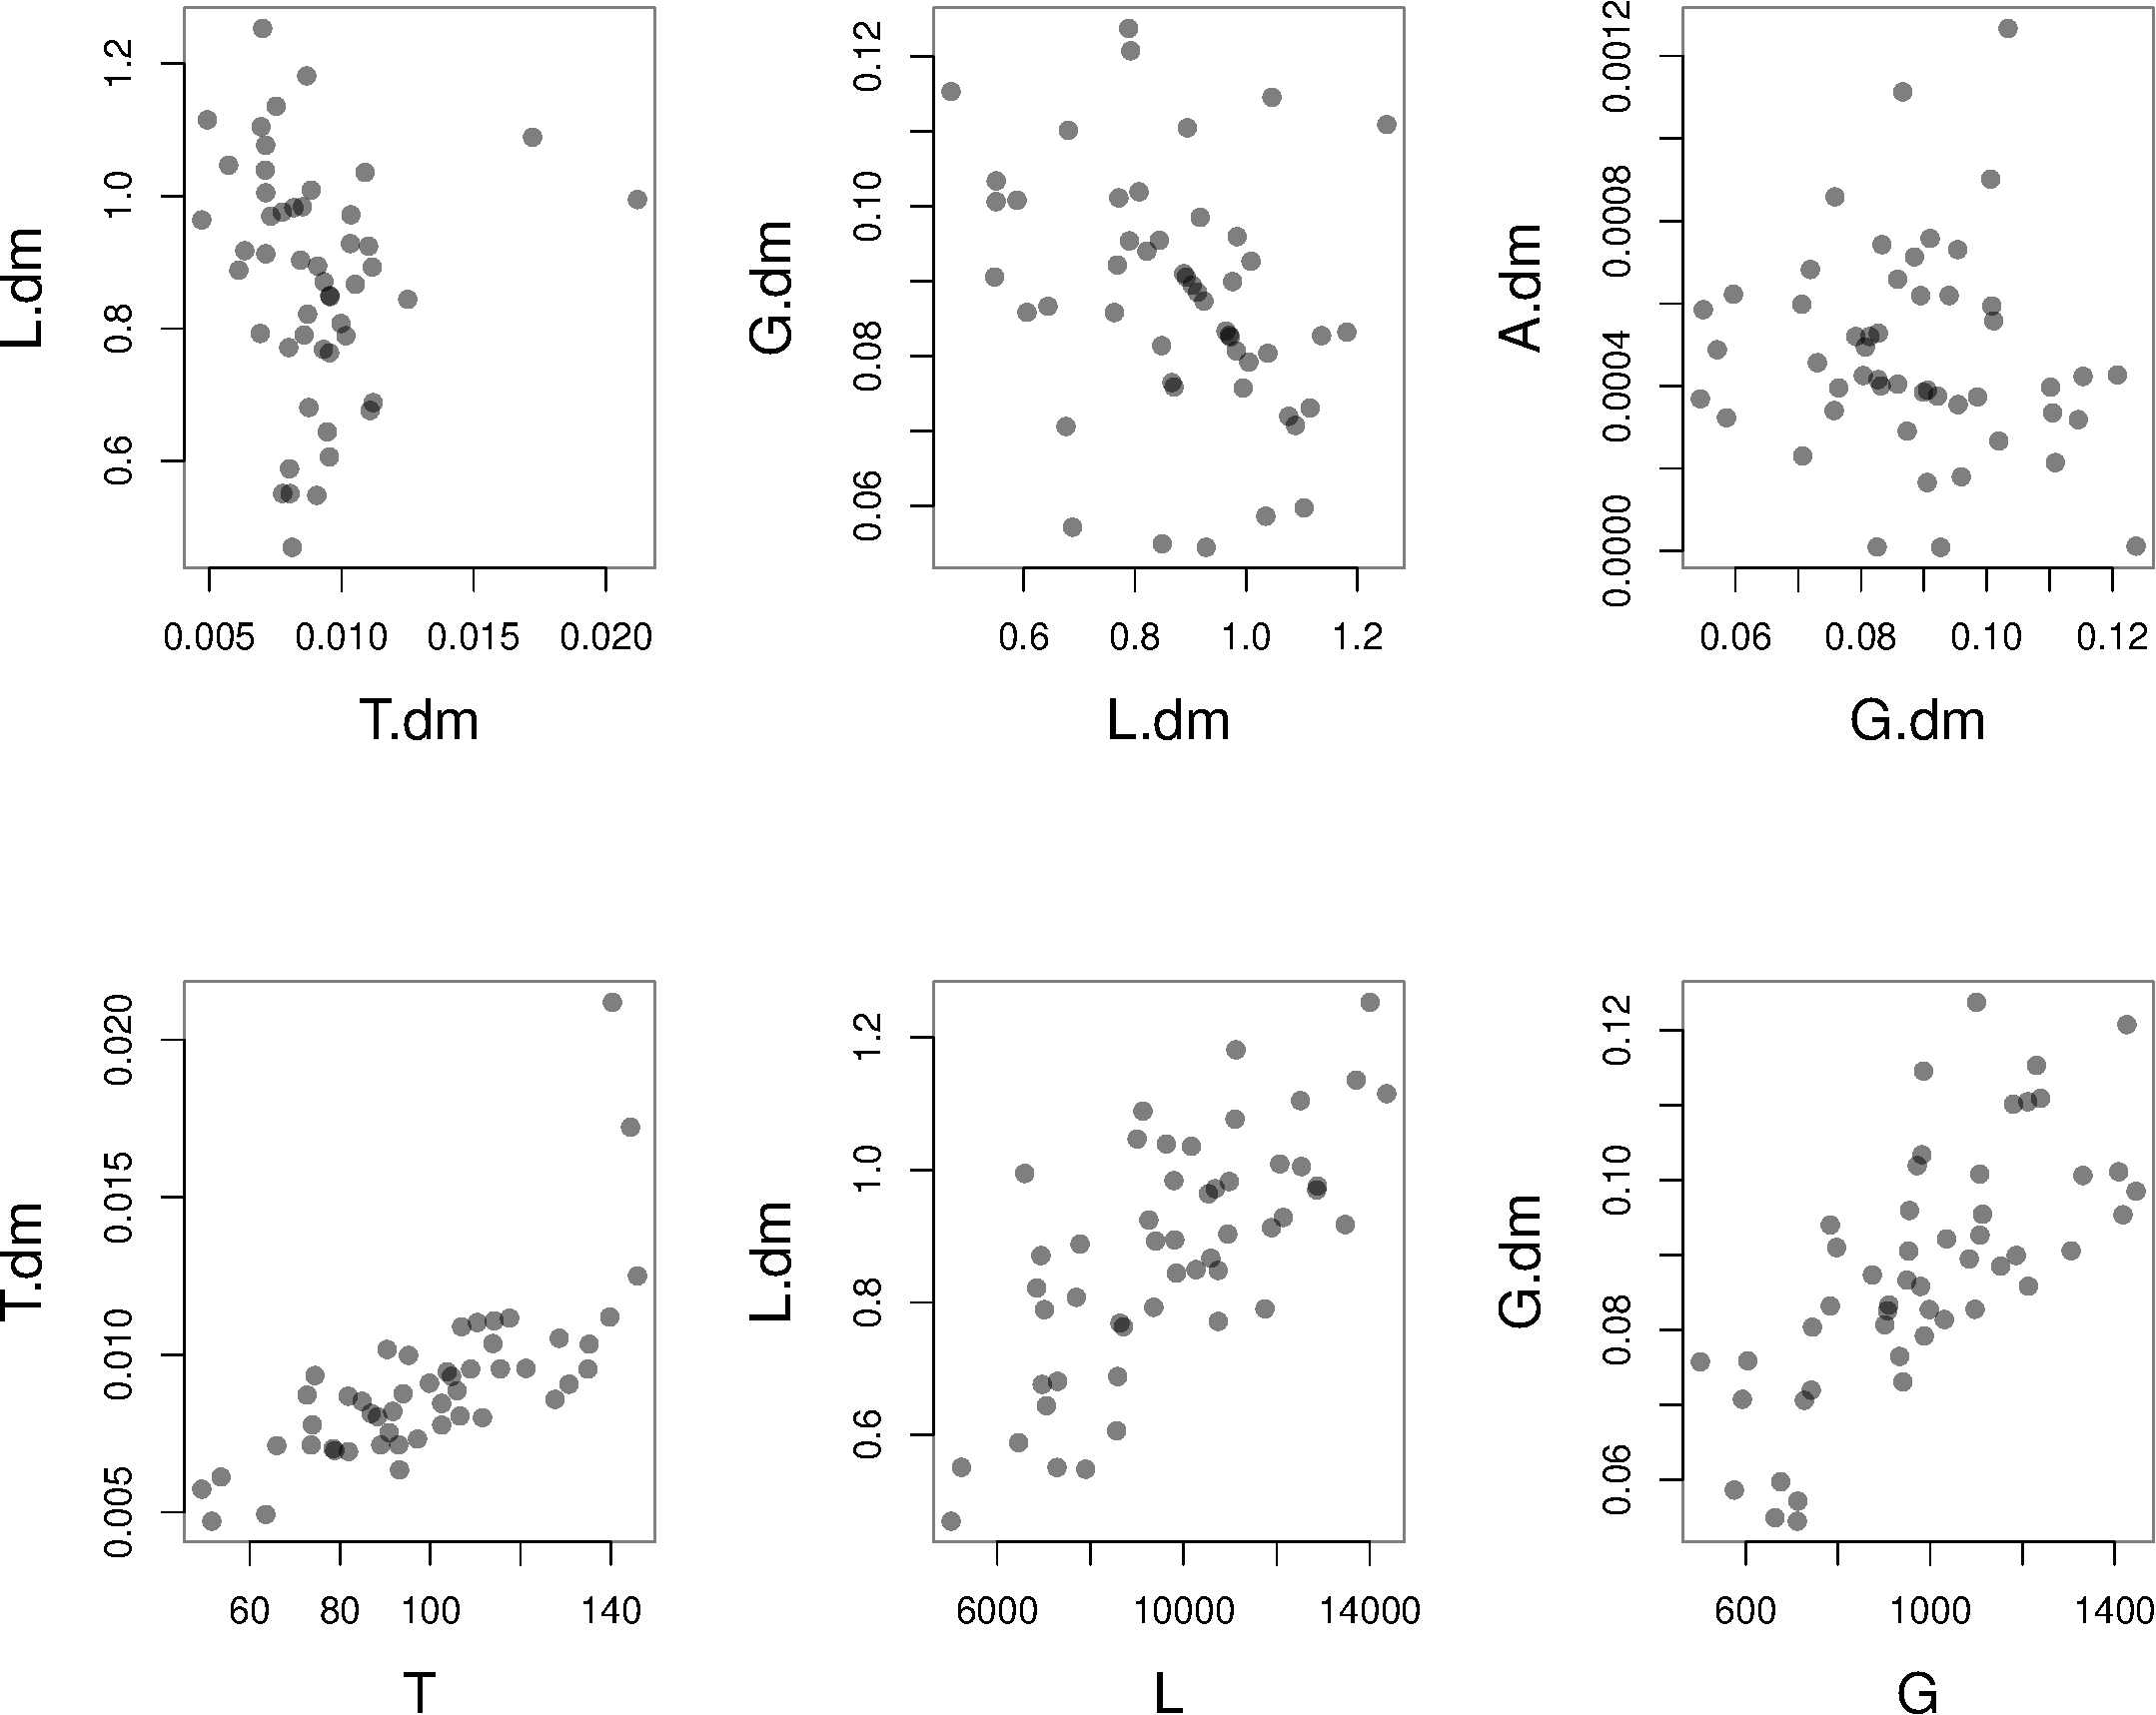
\includegraphics{main_files/figure-latex/R_block_DES-1.pdf}
\caption{\label{numbers} Plot of Ladybugs vs.~Tigers, Gnus vs.~Ladybugs
and Aliens vs.~Gnus for simulated random Normal data after the DM
normalization (top row). Plot of input numerical and DM normalized data
for Tigers, Ladybugs and Gnus (bottom row)}
\end{figure}

This DM transformation at first glance \emph{appears} to fix the problem
caused by converting the data from numbers to proportions. The pairs of
points in the top row are no longer as strongly correlated and the data
seem to be randomly distributed. However, plotting the actual numbers vs
the DM transformed values shows that the DM transformation is not
restoring the data to their original form, but to some other. In the
absence of a solid theoretical foundation, it is difficult to say
exactly how we should interpret these DM-transformed data. It should be
pointed out that above plots were generated on the TSS-normalized
dataset, however only the scale of the \emph{dm} axes would change if
the DM normalization was conducted on the original numerical data. Thus,
conclusions derived from data that are DM-normalized actually tell us
little about the underlying enviroment---despite the pervasive use of
this transformation in the biomedical literature.

\subsection{Log-ratio transformations}\label{log-ratio-transformations}

Aitchison (1986) introduced the concept of the log-ratio transformation.

There are three main log-ratio transformations; the additive log-ratio
(alr), centred log-ratio (clr) and the isometric log-ratio (ilr)
(Aitchison, 1986; Pawlowsky-Glahn et al., 2015).

Using the same notation as above for a sample vector
\(\vec{\textbf{s}}\) of \(D\) `counted' features (taxa, operational
taxonomic units or OTUs, genes, etc.)
\(\vec{\textbf{s}}=[s_1, s_2, ... s_D]\):

The alr is the simply the elements of the sample vector divided by a
presumed invariant feature, which by convention here is the last one:

\begin{equation}
\begin{aligned}
 \vec{\textbf{x}}_{alr}= &\ [log(x_1/x_D), log(x_2/x_D), \\
 & \ldots log(x_D-1/x_D]
\end{aligned}
 \label{eq:alr}
\end{equation}

This is similar to the concept used in quantitative PCR, where the
relative abundance of the feature of interest is divided by the relative
abundance of a (presumed) constant `housekeeping' feature. Of course
there are two major drawbacks. First, that the experimentalist's
knowledge of which, if any, features are invariant is necessarily
incomplete. Second, is that the choice of the (presumed) invariant
feature has a large effect on the result if the presumed invariant
feature is not invariant, or if it is correlated with any other features
in the dataset. Interestingly, an early proposal was to use the
geometric mean of a number of internal controls (Vandesompele et al.,
2002), leading to the next transformation.

The centered log-ratio (clr) transformation introduced by (Aitchison,
1983, 1986) uses the geometric mean of all features as the denominator:

\begin{equation}
\begin{aligned}
   \vec{\textbf{x}}_{clr} = & [log(x_1/\mathrm{G}(\vec{\textbf{x}})), \\
   & log(x_2/\mathrm{G}(\vec{\textbf{x}})), \\
   & \ldots log(x_D/\mathrm{G}(\vec{\textbf{x}}))]
\end{aligned}
\label{eq:clr}
\end{equation}

where
\(\mathrm{G}(\vec{\textbf{x}}) = \sqrt[D]{x_1 \cdot x_2 \cdot ... \cdot x_D}\),
the geometric mean of \(\vec{\textbf{x}}\).

The clr is often criticized since it has the property that the sum of
the clr vector must equal 0. This constraint causes a singular
covariance matrix; i.e., the sum of the covariance matrix is always a
constant (Pawlowsky-Glahn et al., 2015). However the clr has the
advantage of being readily interpretable, a value in the vector is its
abundance \emph{relative} to a mean value.

The ilr is the final transformation, and is a series of sequential
log-ratios between two groups of features. For example, the philr
transformation is the series of ratios between OTUs partitioned along
the phylogenetic tree (Silverman et al., 2017), although any other
sequential binary partitioning scheme is also possible (Pawlowsky-Glahn
et al., 2015). The ilr transformation does not suffer the drawbacks of
either the alr or clr, but does not allow for insights into
relationships between single features in the dataset. Nevertheless, ilr
transformations permit the full-range of multivariate tools to be used,
and are recommended whenever possible.

The ilr and clr are directly comparable in a two important ways: First,
the distances between samples computed using an ilr and clr
transformation are equivalent. Second, the clr approaches the ilr in
other respects as the number of features becomes large. In this respect,
the large number of features---hundreds in the case of OTUs, thousands
in the case of genes---in a typical experiment works in our favour.
Thus, while not perfect, the clr is the most widely used transformation.
However, care must be taken when interpreting its outputs since single
features must always be interpreted as a ratio between the feature and
the denominator used for the clr transformation. The problems of using
clr are apparent when some subcomposition or group of taxa is analysed
for further insight since the geometric mean of the subcomposition is
not necessarily equal to that of the original composition, leading to
potential inconsistencies.

Log-ratio values of any type do not need to be normalized since the
total sum is a term in both the numerator and the denominator. Thus, the
same log-ratio value will be obtained for the vector of raw read counts,
or the vector of normalized read counts, or the vector of proportions
calculated from the counts. Thus, log-ratios are said to be equivalence
classes such that there is no information in the total count (aside from
precision) (Barceló-Vidal et al., 2001).

Attempts to `open' the data are doomed to failure because the data
cannot be moved from the simplex to Euclidian space. The total count
delivered by the sequencing instrument is a function of the instrument
and not the number of molecules sampled from the environment, thus the
total count has no geometric meaning. If the data are collected in such
a way that the total count represents the actual count in the
environment, then the data are not compositional and issues regarding
compositional data disappear. However, at present all sequencing
platforms deliver a fixed-sum, random sample of the proportion of
molecules in the environment.

Note that this does not mean that the read depth is irrelevant since
more reads for a sample translate into greater precision when estimating
the proportions (Fernandes et al., 2013).

\section{Comparing Transforms and Distances}

The microbiome and transcriptome literature are replete with distance
metrics, and it is common to find that a single study will use several
distance metrics to report their findings. This is a problem since it
shows that practitioners are unsure of the reason to use a metric, and
the use of more than one metric leads to data dredging and research
degrees of freedom---both of which increase the chances of finding false
positives in the data to a surety.

Distance metrics can be broadly divided into those that require
partitioning and those that do not. The UniFrac (Lozupone and Knight,
2005; Lozupone et al., 2011) and philr (Silverman et al., 2017) both
require a phylogenetic tree, making these metrics applicable only to
situations where the features can be so partitioned. For example, these
distances are useful when examining 16S rRNA gene sequencing
experiments. We have found that the unweighted UniFrac method is
unreliable, and should be used with caution {[}Wong et al. (2016)\}, a
point that was made in the original UniFrac paper and subsequently
forgotten. The philr metric is a drop-in replacement for the weighted
UniFrac distance metric and should be used whenever possible, since
\texttt{philr} is an ilr transformation of the data where the sequential
binary partitions are made along the phylogenetic tree. The
\texttt{philr} transformation is thus compositionally appropriate. In
practice, the weighted UniFrac distance metric provides similar results
to the Aitchison distance, described below, and the ilr distance
calculated using the philr transform approaches the Aitchison distance
when the number of features is large.

Several non-phylogenetic distances are in widespread use in the
literature. These will be discussed in turn below, and their effects on
distances between a random samples illustrated.

\subsection{Distances in counts and proportion}

Ideally, we use distance metrics to inform us as to something of
relevance in the actual sample. That is, if we collect our data on the
numbers of tigers, ladybugs, gnus and space aliens, what can we infer
about the actual data \emph{after  sequencing}? which as we have seen,
is the same as asking what can we infer after converting the data to
relative abundances (proportions)?

There are two main ways to think about distances: Euclidian and
Manhattan. The Euclidian distance is the straight-line distance between
two points. If we have a rectangular room, the Euclidian distance
between two corners would be the distance travelled by walking
diagonally across the room from one corner to the other. The Manhattan
distance would be the distance travelled by walking along the walls
between the two corners. Obviously, the Manhattan distance will always
be larger than the Euclidian distance. So how do these two simple
metrics compare when calculate on numbers and on compositions?

\begin{Shaded}
\begin{Highlighting}[]
\KeywordTok{library}\NormalTok{(vegan)}

\NormalTok{dist.ran.dat <-}\StringTok{ }\KeywordTok{as.matrix}\NormalTok{(}\KeywordTok{vegdist}\NormalTok{(}
    \NormalTok{ran.dat, }\DataTypeTok{method=}\StringTok{"euclidian"}\NormalTok{))}
\NormalTok{dist.ran.dat.MAN <-}\StringTok{ }\KeywordTok{as.matrix}\NormalTok{(}\KeywordTok{vegdist}\NormalTok{(}
    \NormalTok{ran.dat, }\DataTypeTok{method=}\StringTok{"manhattan"}\NormalTok{))}
\NormalTok{dist.ran.dat.prop <-}\StringTok{ }\KeywordTok{as.matrix}\NormalTok{(}\KeywordTok{vegdist}\NormalTok{(}
    \NormalTok{ran.dat.prop, }\DataTypeTok{method=}\StringTok{"euclidian"}\NormalTok{))}
\NormalTok{dist.ran.dat.prop.MAN <-}\StringTok{ }\KeywordTok{as.matrix}\NormalTok{(}\KeywordTok{vegdist}\NormalTok{(}
    \NormalTok{ran.dat.prop, }\DataTypeTok{method=}\StringTok{"manhattan"}\NormalTok{))}

\KeywordTok{par}\NormalTok{(}\DataTypeTok{mfrow=}\KeywordTok{c}\NormalTok{(}\DecValTok{2}\NormalTok{,}\DecValTok{2}\NormalTok{), }\DataTypeTok{pch=}\DecValTok{19}\NormalTok{, }\DataTypeTok{col=}\KeywordTok{rgb}\NormalTok{(}\DecValTok{0}\NormalTok{,}\DecValTok{0}\NormalTok{,}\DecValTok{0}\NormalTok{,}\FloatTok{0.5}\NormalTok{),}
    \DataTypeTok{cex=}\FloatTok{1.5}\NormalTok{, }\DataTypeTok{cex.lab=}\FloatTok{1.5}\NormalTok{)}

\KeywordTok{plot}\NormalTok{(dist.ran.dat[}\DecValTok{1}\NormalTok{,], dist.ran.dat.MAN[}\DecValTok{1}\NormalTok{,],}
    \DataTypeTok{xlab=}\StringTok{"Euclidian"}\NormalTok{, }\DataTypeTok{ylab=}\StringTok{"Manhatten"}\NormalTok{,}
    \DataTypeTok{main=}\StringTok{"Numbers"}\NormalTok{)}
\KeywordTok{plot}\NormalTok{(dist.ran.dat.prop[}\DecValTok{1}\NormalTok{,], dist.ran.dat.prop.MAN[}\DecValTok{1}\NormalTok{,],}
    \DataTypeTok{xlab=}\StringTok{"Euclidian.p"}\NormalTok{, }\DataTypeTok{ylab=}\StringTok{"Manhattan.p"}\NormalTok{,}
    \DataTypeTok{main=}\StringTok{"Proportions"}\NormalTok{)}
\KeywordTok{plot}\NormalTok{(dist.ran.dat[}\DecValTok{1}\NormalTok{,], dist.ran.dat.prop[}\DecValTok{1}\NormalTok{,],}
    \DataTypeTok{xlab=}\StringTok{"Euclidian"}\NormalTok{, }\DataTypeTok{ylab=}\StringTok{"Euclidian.p"}\NormalTok{,}
    \DataTypeTok{main=}\StringTok{"Number vs Proportions"}\NormalTok{)}
\KeywordTok{plot}\NormalTok{(dist.ran.dat.MAN[}\DecValTok{1}\NormalTok{,], dist.ran.dat.prop.MAN[}\DecValTok{1}\NormalTok{,],}
    \DataTypeTok{xlab=}\StringTok{"Manhattan"}\NormalTok{, }\DataTypeTok{ylab=}\StringTok{"Manhattan.p"}\NormalTok{,}
    \DataTypeTok{main=}\StringTok{"Number vs Proportions"}\NormalTok{)}
\end{Highlighting}
\end{Shaded}

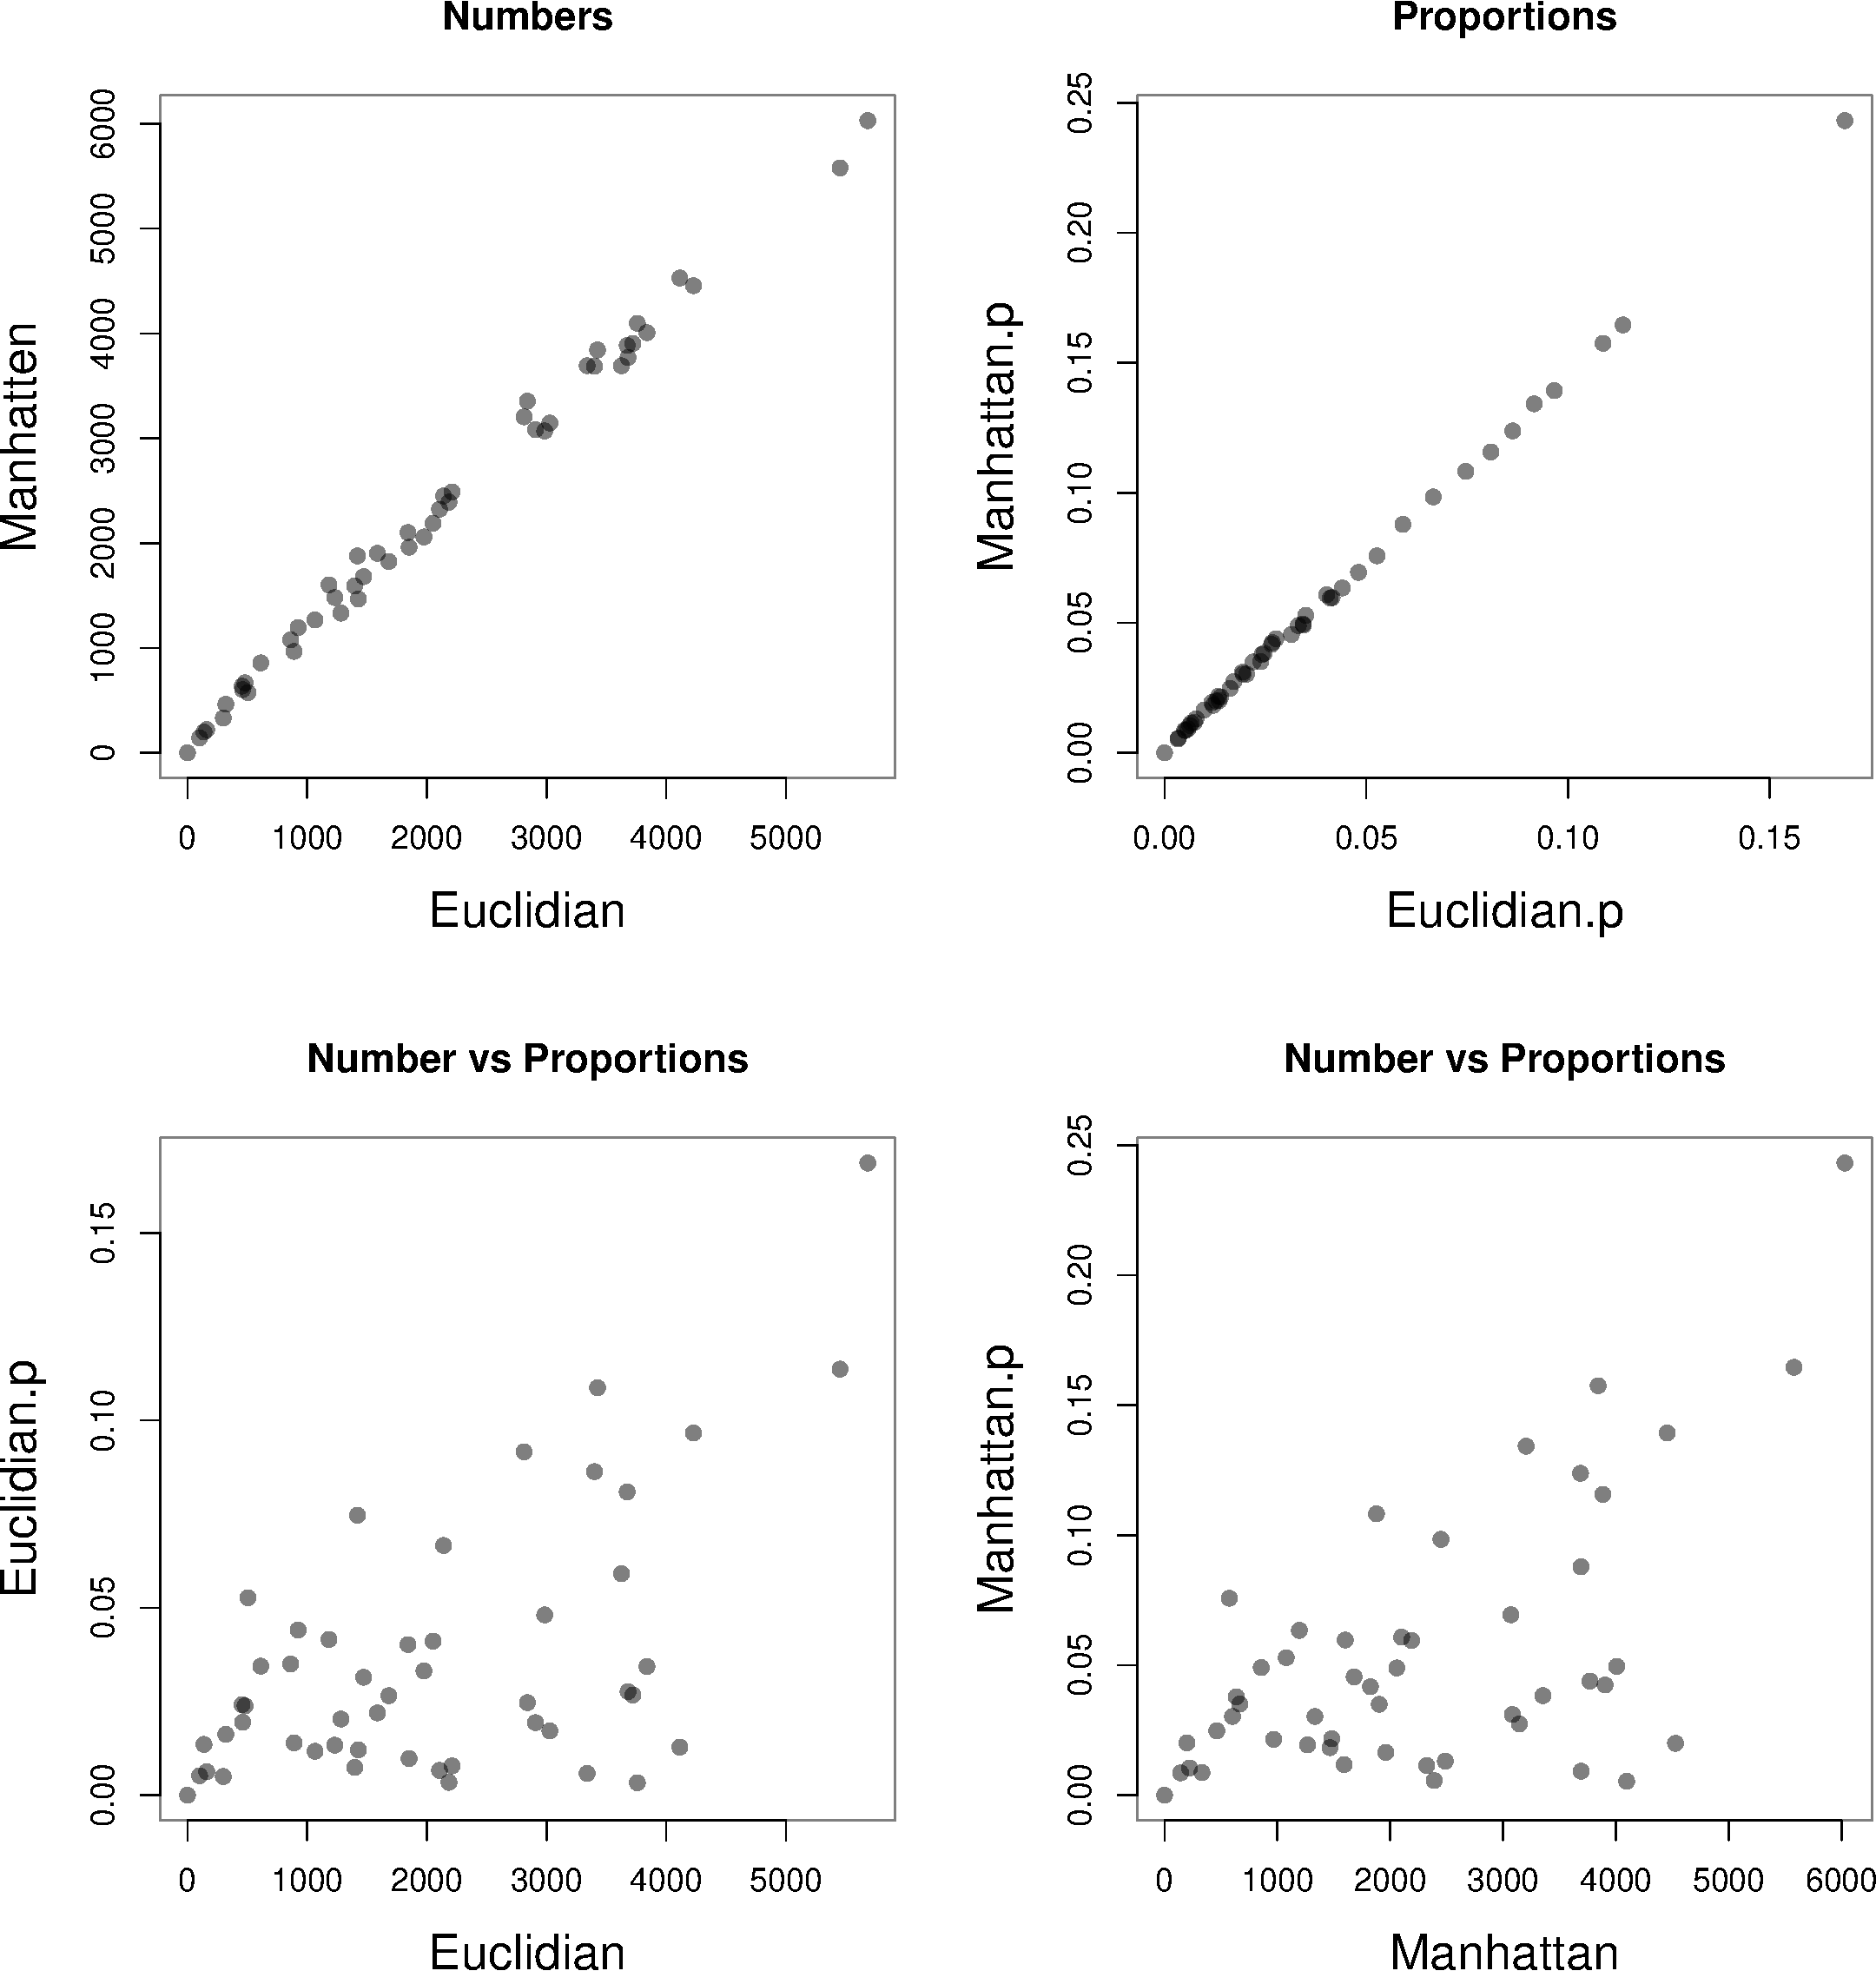
\includegraphics{main_files/figure-latex/R_block_dist-1.pdf}

We can see that the Euclidian and Manhattan distances are generally
correlated, but not identical, when comparing distances in the original
set of random samples only, or when the data in the samples are
converted to proportions. However, the distances between samples are
very different when comparing the numerical and proportional data. This
tells us that the inferences we make from sequencing data can not
translate to inferences about the actual abundances of features in the
environment, but only to their relative abundances. So which distance
metric should we use for proportional data? It turns out that neither
are suitable because these distance metrics assume linear differences
between features, and this is not true in proportional data (Aitchison,
1986).

Data normalizations are often touted as removing the compositionality of
the data. We shall see that this is not true, and inappropriate data
transformations confound, rather than providing clarity.

Plotting three of the possible combinations, we can see that the
features are essentially uncorrelated with each other and each sample is
a random distances from any other. Any inference we make from
transformations of this data must be relatable to this `ground truth'. I
now run through each of the transformations in turn, and illustrate the
difference between the actual data, and the transformed data.

\subsection{Bray-Curtis Dissimilarity}

The Bray-Curtis dissimilarity is a Manhattan distance normalized to
range between 0 and 1. In the test dataset, the Euclidian distance and
the Bray-Curtis (BC) distances are essentially linearly related.

\begin{Shaded}
\begin{Highlighting}[]
\KeywordTok{library}\NormalTok{(vegan)}

\NormalTok{dist.ran.dat.BC <-}\StringTok{ }\KeywordTok{as.matrix}\NormalTok{(}\KeywordTok{vegdist}\NormalTok{(}
    \NormalTok{ran.dat, }\DataTypeTok{method=}\StringTok{"bray"}\NormalTok{))}
\NormalTok{dist.ran.dat.MAN <-}\StringTok{ }\KeywordTok{as.matrix}\NormalTok{(}\KeywordTok{vegdist}\NormalTok{(}
    \NormalTok{ran.dat, }\DataTypeTok{method=}\StringTok{"manhattan"}\NormalTok{))}
\NormalTok{dist.ran.dat.DM.BC <-}\StringTok{ }\KeywordTok{as.matrix}\NormalTok{(}\KeywordTok{vegdist}\NormalTok{(}
    \NormalTok{ran.dat.DM, }\DataTypeTok{method=}\StringTok{"bray"}\NormalTok{))}
\NormalTok{dist.ran.dat.prop.BC <-}\StringTok{ }\KeywordTok{as.matrix}\NormalTok{(}\KeywordTok{vegdist}\NormalTok{(}
    \NormalTok{ran.dat.prop, }\DataTypeTok{method=}\StringTok{"bray"}\NormalTok{))}

\KeywordTok{par}\NormalTok{(}\DataTypeTok{mfrow=}\KeywordTok{c}\NormalTok{(}\DecValTok{2}\NormalTok{,}\DecValTok{2}\NormalTok{), }\DataTypeTok{pch=}\DecValTok{19}\NormalTok{, }\DataTypeTok{col=}\KeywordTok{rgb}\NormalTok{(}\DecValTok{0}\NormalTok{,}\DecValTok{0}\NormalTok{,}\DecValTok{0}\NormalTok{,}\FloatTok{0.5}\NormalTok{),}
    \DataTypeTok{cex=}\FloatTok{1.5}\NormalTok{, }\DataTypeTok{cex.lab=}\FloatTok{1.5}\NormalTok{)}

\KeywordTok{plot}\NormalTok{(dist.ran.dat.MAN[}\DecValTok{1}\NormalTok{,],dist.ran.dat[}\DecValTok{1}\NormalTok{,],}
    \DataTypeTok{xlab=}\StringTok{"S1 Euc"}\NormalTok{, }\DataTypeTok{ylab=}\StringTok{"S1 BC"}\NormalTok{,}
    \DataTypeTok{main=}\StringTok{"Euc vs BC"}\NormalTok{)}
\KeywordTok{plot}\NormalTok{(dist.ran.dat.BC[}\DecValTok{1}\NormalTok{,], dist.ran.dat.prop.BC[}\DecValTok{1}\NormalTok{,],}
    \DataTypeTok{xlab=}\StringTok{"S1 BC"}\NormalTok{, }\DataTypeTok{ylab=}\StringTok{"S1.p BC"}\NormalTok{,}
    \DataTypeTok{main=}\StringTok{"BC vs BC.p"}\NormalTok{)}
\KeywordTok{plot}\NormalTok{(dist.ran.dat.BC[}\DecValTok{1}\NormalTok{,], dist.ran.dat.DM.BC[}\DecValTok{1}\NormalTok{,],}
    \DataTypeTok{xlab=}\StringTok{"S1 BC"}\NormalTok{, }\DataTypeTok{ylab=}\StringTok{"S1.p DM"}\NormalTok{,}
    \DataTypeTok{main=}\StringTok{"BC vs BC.DM"}\NormalTok{)}
\KeywordTok{plot}\NormalTok{(dist.ran.dat.prop.BC[}\DecValTok{1}\NormalTok{,], dist.ran.dat.DM.BC[}\DecValTok{1}\NormalTok{,],}
    \DataTypeTok{xlab=}\StringTok{"S1.p BC"}\NormalTok{, }\DataTypeTok{ylab=}\StringTok{"S1.p DM"}\NormalTok{,}
    \DataTypeTok{main=}\StringTok{"BC.p vs BC.DM"}\NormalTok{)}
\end{Highlighting}
\end{Shaded}

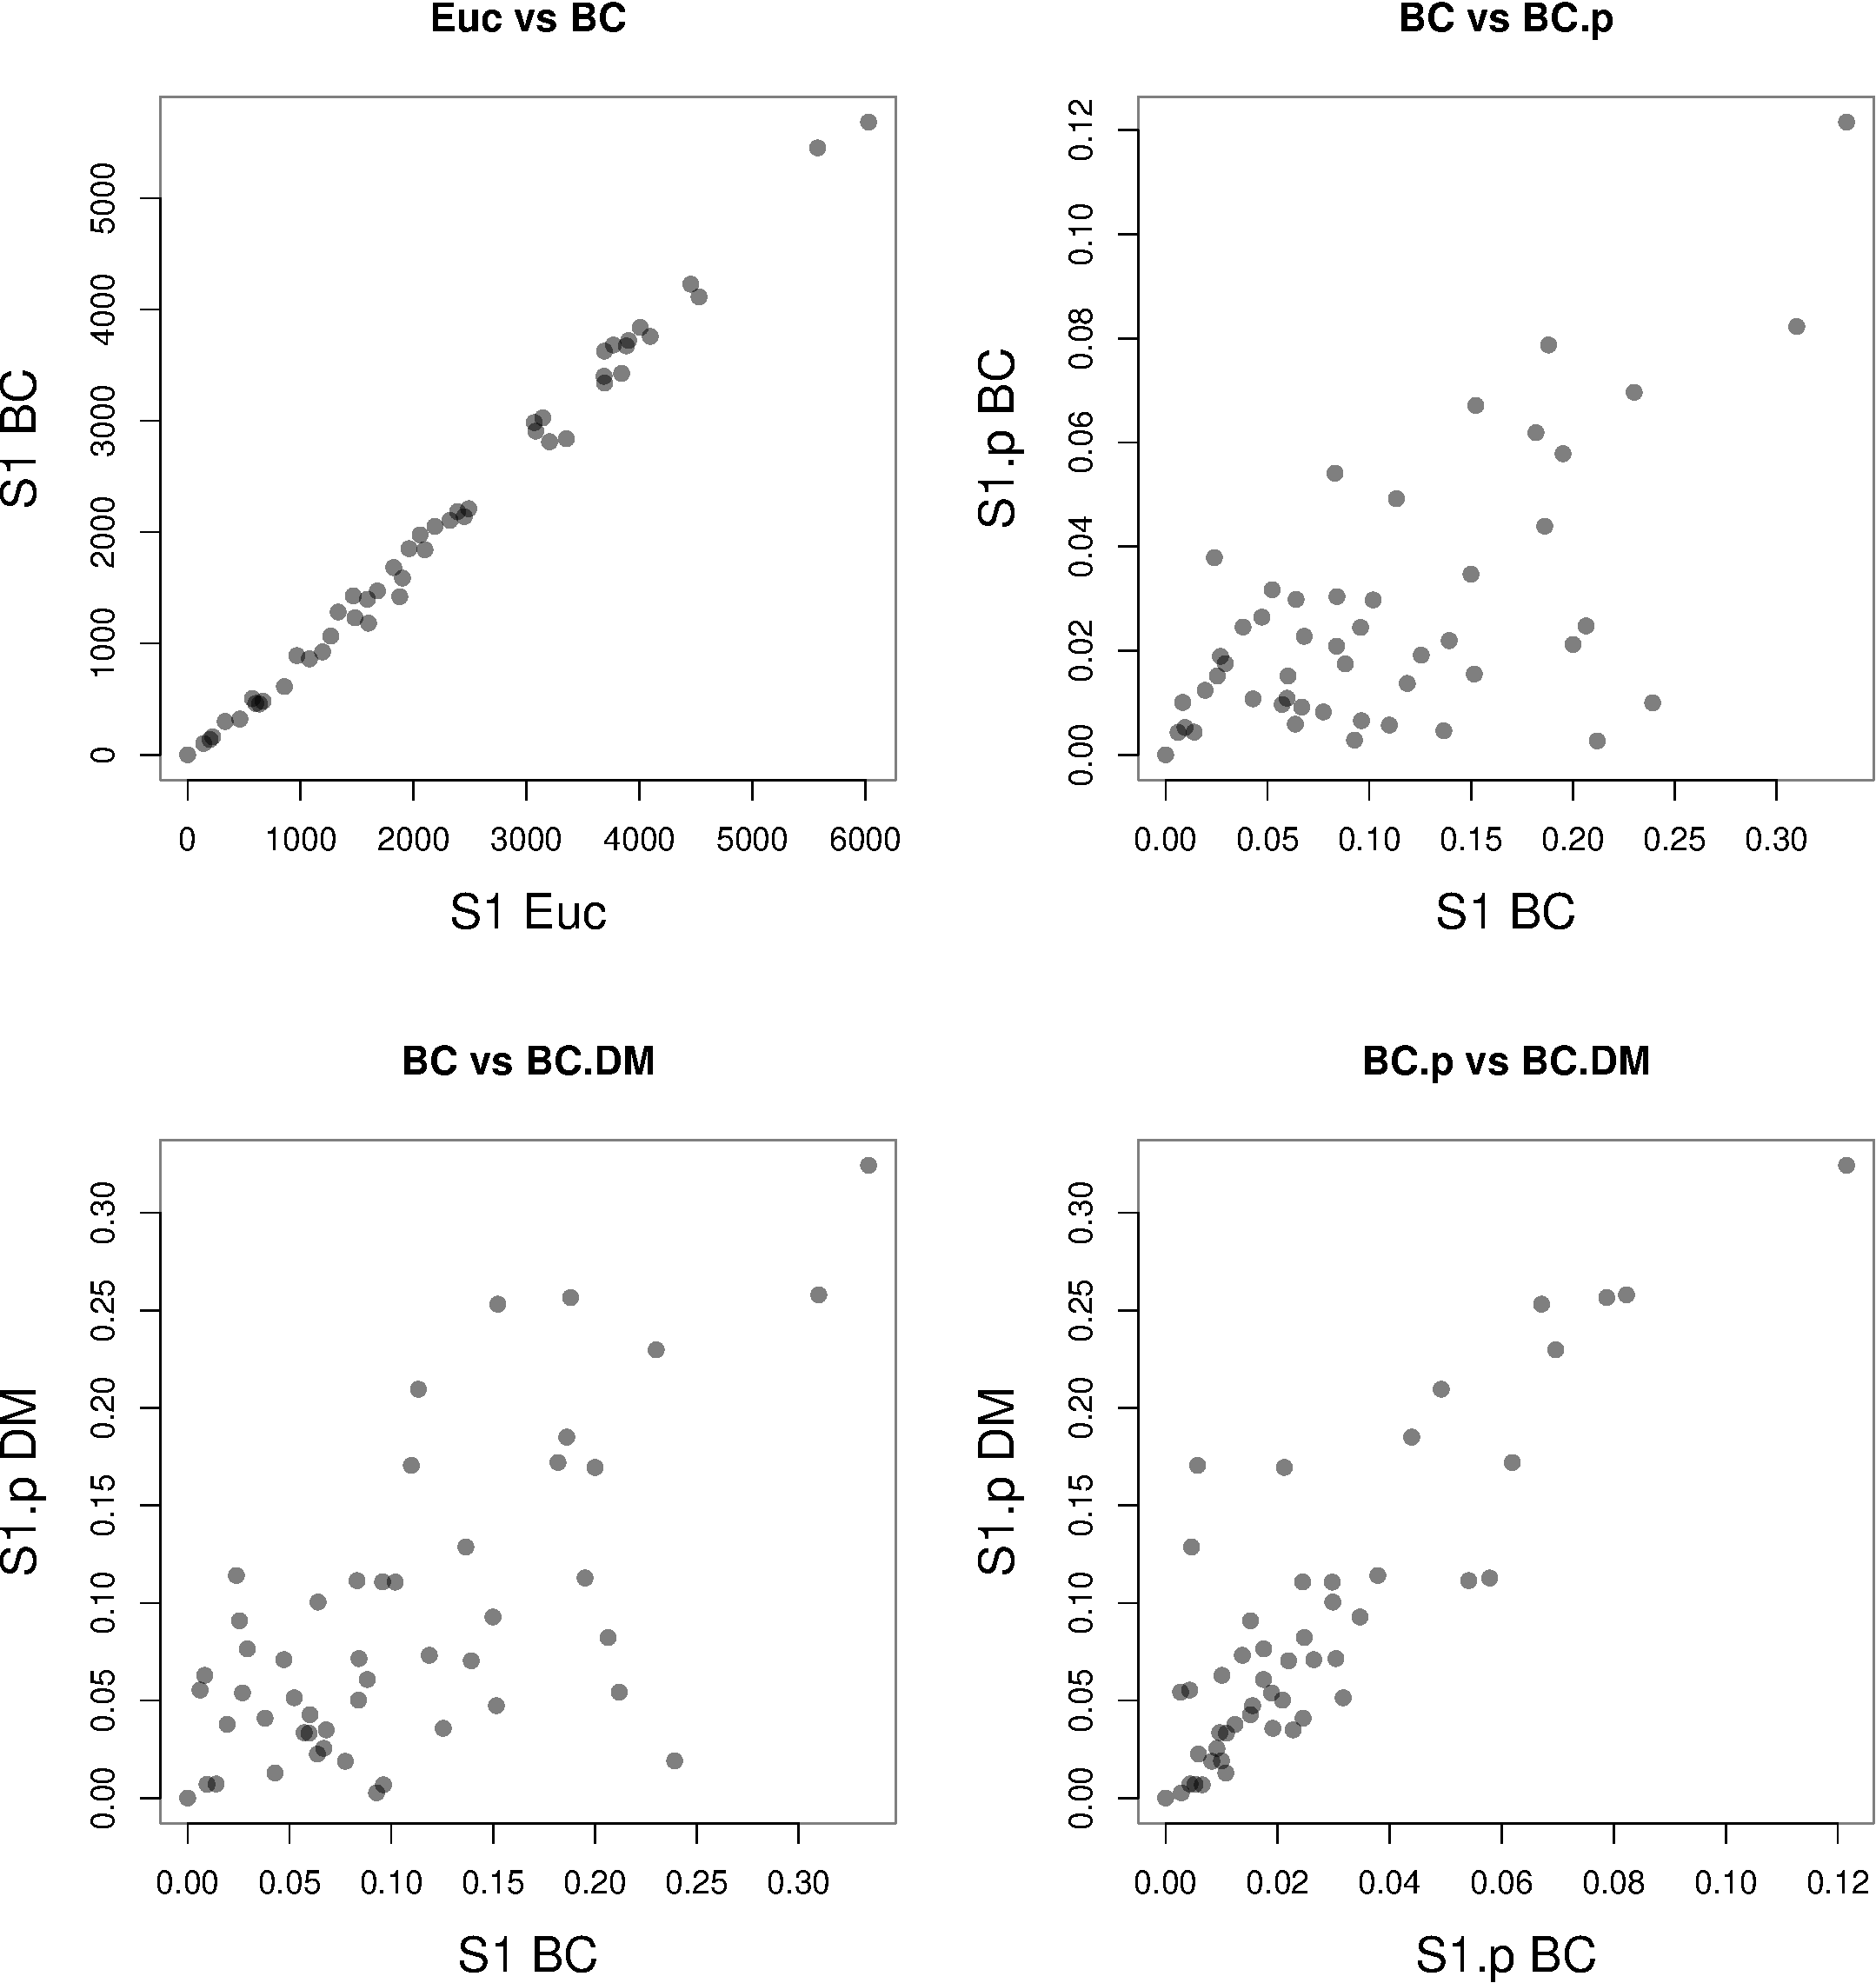
\includegraphics{main_files/figure-latex/R_block_bray-1.pdf}

\subsection{Euclidian Distance of TSS scaling transformation}

The TSS scaling transformation is simply a conversion of each sample
from a count to a proportion.

\begin{Shaded}
\begin{Highlighting}[]
\NormalTok{dist.ran.dat.prop <-}\StringTok{ }\KeywordTok{as.matrix}\NormalTok{(}\KeywordTok{dist}\NormalTok{(}
    \NormalTok{ran.dat.prop, }\DataTypeTok{method=}\StringTok{"euclidian"}\NormalTok{))}
\end{Highlighting}
\end{Shaded}

\subsection{Euclidian Distance of DM transformation}

The DM scaling transformation is a change in the scale of the sample
vector \(\vect{j}\), where each sample is scaled by a different amount.
This has the desirable property that it \emph{can} restore the a
conversion of each sample from a count to a proportion.

\begin{Shaded}
\begin{Highlighting}[]
\NormalTok{dist.ran.dat.DM <-}\StringTok{ }\KeywordTok{as.matrix}\NormalTok{(}\KeywordTok{dist}\NormalTok{(}
    \NormalTok{ran.dat.DM, }\DataTypeTok{method=}\StringTok{"euclidian"}\NormalTok{))}

\KeywordTok{par}\NormalTok{(}\DataTypeTok{mfrow=}\KeywordTok{c}\NormalTok{(}\DecValTok{2}\NormalTok{,}\DecValTok{2}\NormalTok{), }\DataTypeTok{pch=}\DecValTok{19}\NormalTok{, }\DataTypeTok{col=}\KeywordTok{rgb}\NormalTok{(}\DecValTok{0}\NormalTok{,}\DecValTok{0}\NormalTok{,}\DecValTok{0}\NormalTok{,}\FloatTok{0.5}\NormalTok{),}
    \DataTypeTok{cex=}\FloatTok{1.5}\NormalTok{, }\DataTypeTok{cex.lab=}\FloatTok{1.5}\NormalTok{)}

\KeywordTok{plot}\NormalTok{(ran.dat.DM[,}\StringTok{"T"}\NormalTok{],ran.dat.DM[,}\StringTok{"L"}\NormalTok{],}
    \DataTypeTok{xlab=}\StringTok{"T.dm"}\NormalTok{, }\DataTypeTok{ylab=}\StringTok{"L.dm"}\NormalTok{)}
\KeywordTok{plot}\NormalTok{(ran.dat.DM[,}\StringTok{"L"}\NormalTok{],ran.dat.DM[,}\StringTok{"G"}\NormalTok{],}
    \DataTypeTok{xlab=}\StringTok{"L.dm"}\NormalTok{, }\DataTypeTok{ylab=}\StringTok{"G.dm"}\NormalTok{)}
\KeywordTok{plot}\NormalTok{(ran.dat.DM[,}\StringTok{"G"}\NormalTok{],ran.dat.DM[,}\StringTok{"A"}\NormalTok{],}
    \DataTypeTok{xlab=}\StringTok{"G.dm"}\NormalTok{, }\DataTypeTok{ylab=}\StringTok{"A.dm"}\NormalTok{)}
\KeywordTok{plot}\NormalTok{(dist.ran.dat[}\DecValTok{1}\NormalTok{,], dist.ran.dat.DM[}\DecValTok{1}\NormalTok{,],}
    \DataTypeTok{xlab=}\StringTok{"S1 vs all"}\NormalTok{, }\DataTypeTok{ylab=}\StringTok{"S1.dm vs all.dm"}\NormalTok{,}
    \DataTypeTok{main=}\StringTok{"Distance"}\NormalTok{)}
\end{Highlighting}
\end{Shaded}

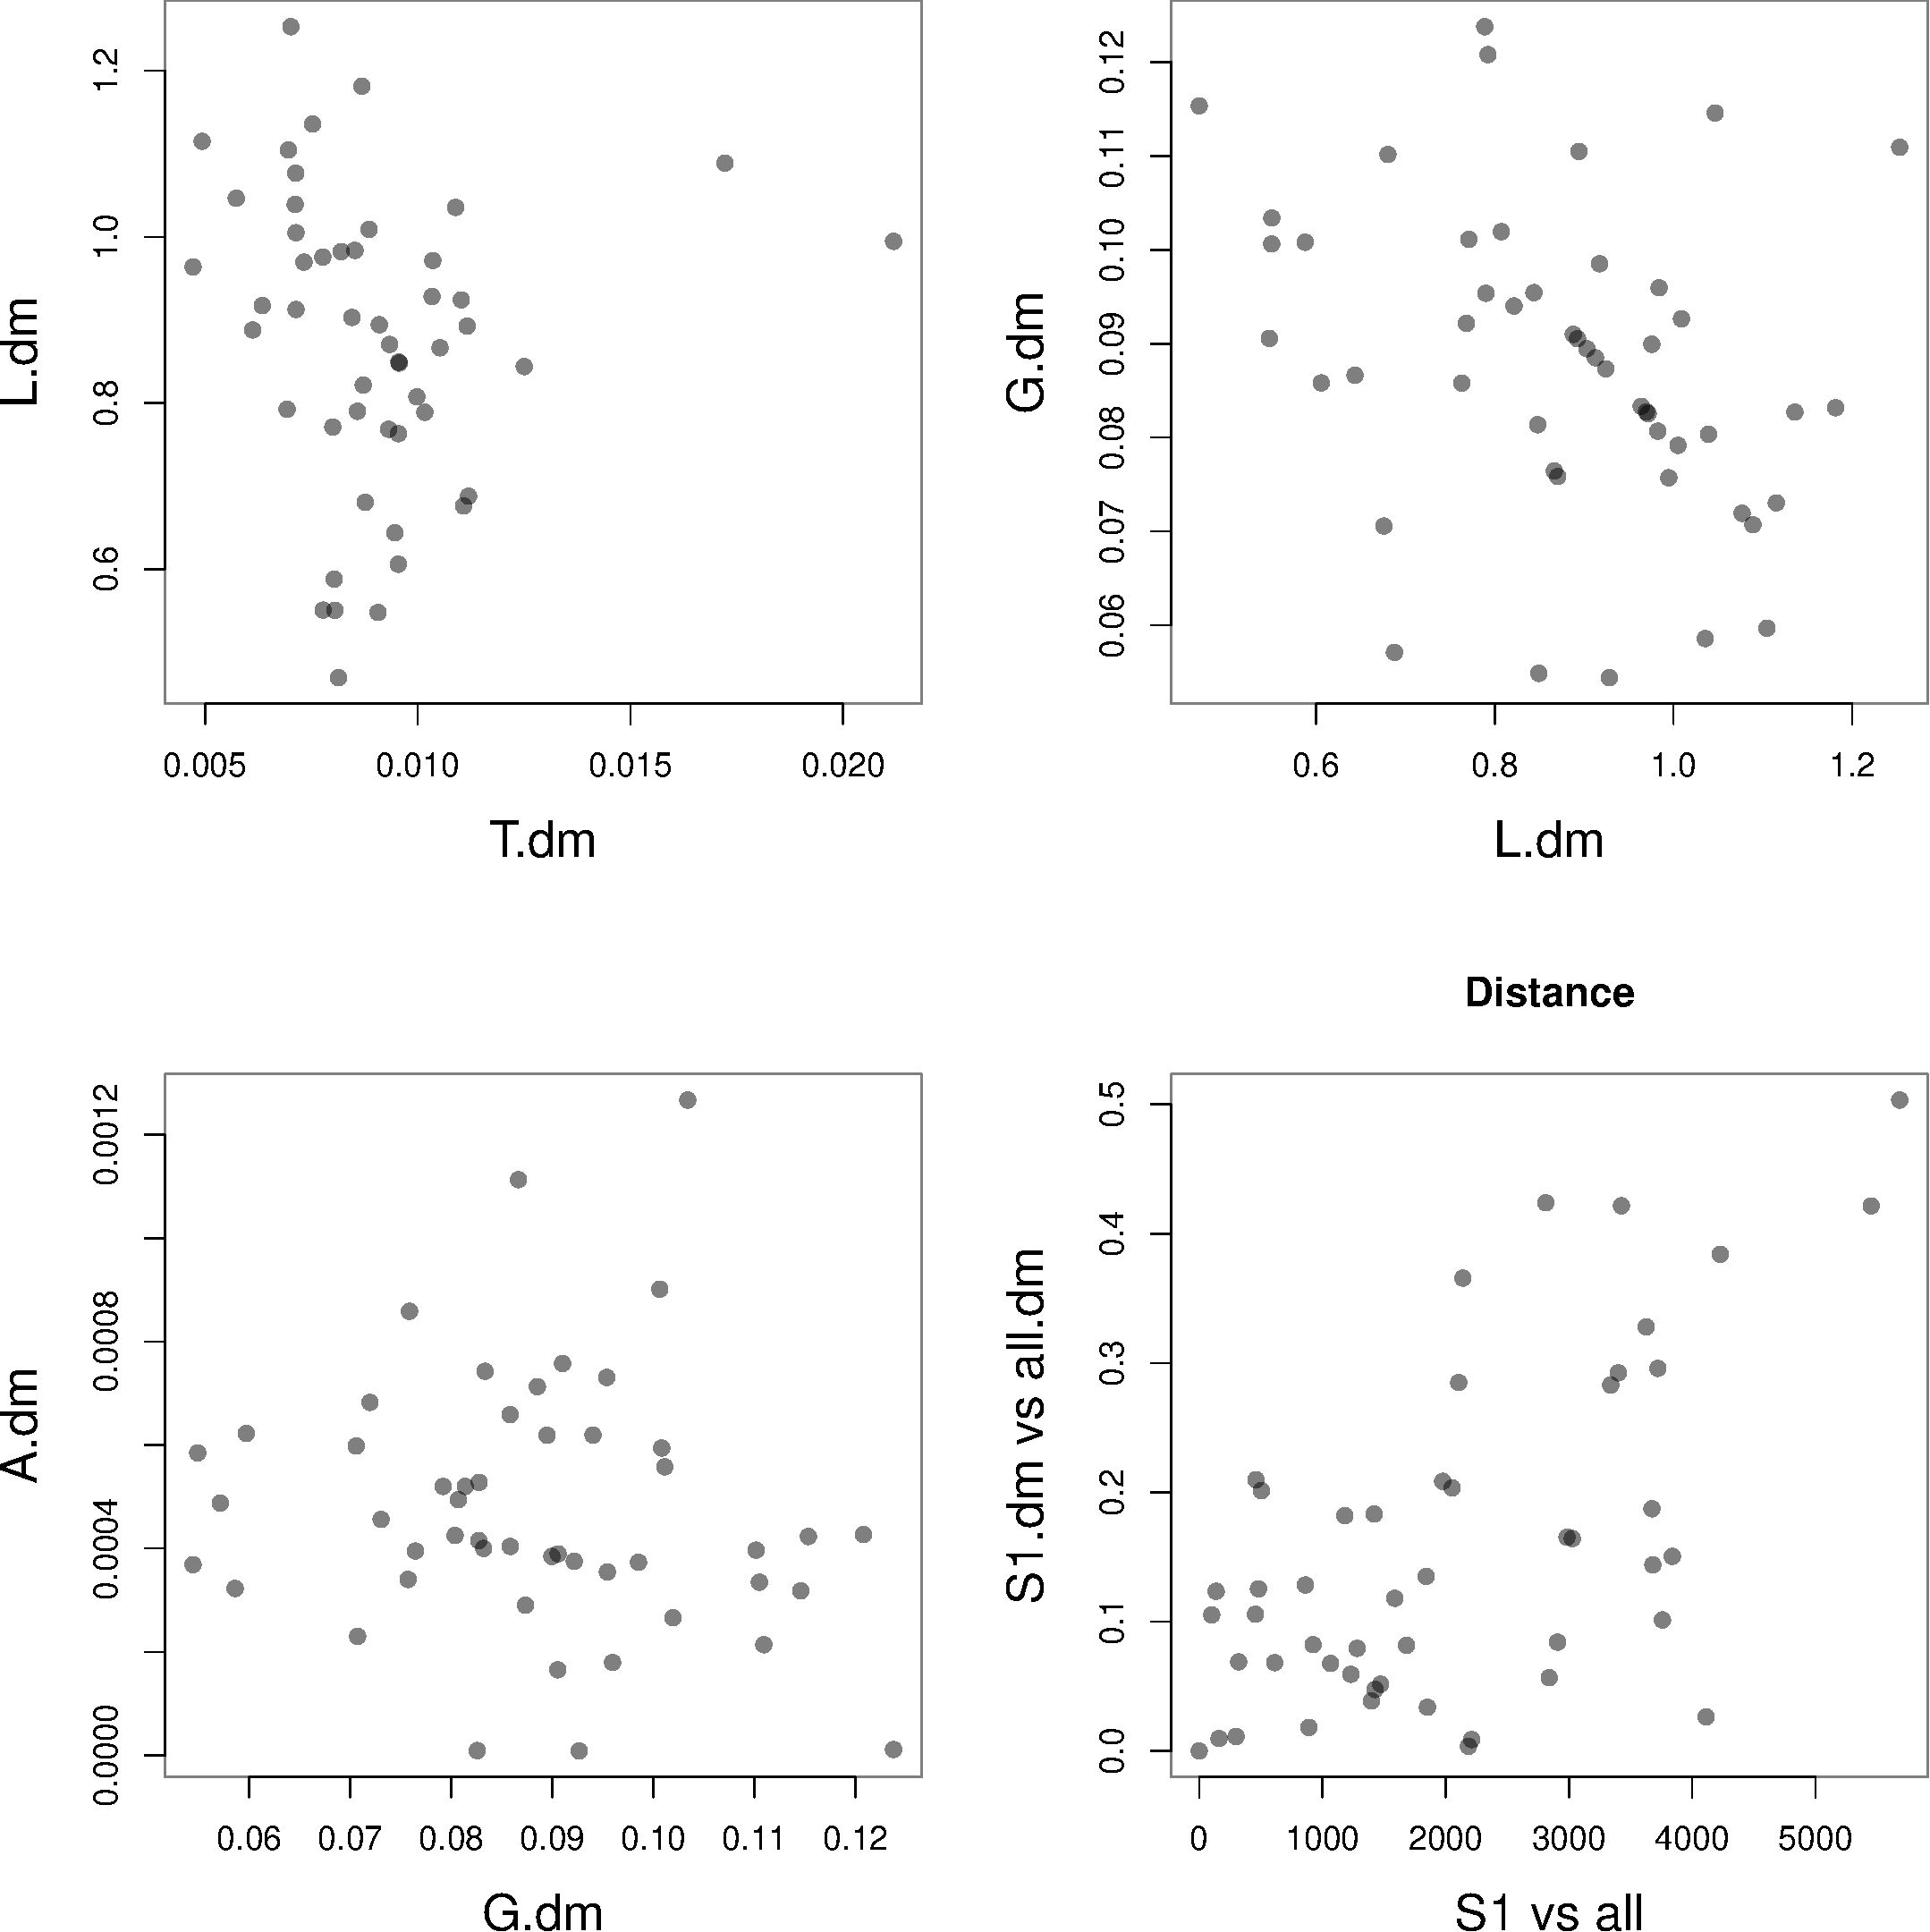
\includegraphics{main_files/figure-latex/R_block_random_DM-1.pdf}

\texttt{plot\_ly(x=ran.dat[,"L"], y=ran.dat[,"T"], z=ran.dat[,"G"])}

\texttt{plot\_ly(x=ran.dat.prop[,"L"], y=ran.dat.prop[,"T"], z=ran.dat.prop[,"G"])}

\texttt{plot\_ly(x=ran.dat.DM[,"L"], y=ran.dat.DM[,"T"], z=ran.dat.DM[,"G"])}

\subsection{Jensen-Shannon Divergence}\subsection{Aitchison Distance}

\section{Exploring compositional data: the compositional
biplot}\label{exploring-compositional-data-the-compositional-biplot}

There are three main data analysis issues that must be acknowledged.

First, the nature of these data are misunderstood. As outlined above,
the number of counts observed per OTU are determined entirely by the
capacity of the instrument and provide no information about the number
of molecules in the input sample. Recall that both bacterial growth, and
PCR are doubling processes and not linear processes, and so would be
better modelled as log\(_2\) differences.

Understanding that we are dealing with fold-change data is an explicit
acknowledgement that the data do not map to normal Euclidian space where
differences are linear. Commonly used statistical tests expect linear
differences between values and so are compromised to some degree, often
catastrophically(Aitchison, 1986,vandenBoogaart2008320) Therefore, the
often-used approaches of converting the OTU count values to proportions
or percentages and conducting statistical tests on those values, or of
using data reduction strategies such as Principle Component Analysis on
the values are inappropriate because the differences between values are
not linear. An alternative approach is to convert the OTU counts to
ratios(Aitchison, 1986; Aitchison and J. Egozcue, 2005; Pawlowsky-Glahn
and Buccianti, 2011; Pawlowsky-Glahn and Egozcue, 2006) which makes the
differences between the ratios of values linear, and so allows the use
of common statistical tests.

However the user must interpret the output as ratios between feature
abundances rather than absolute differences(Pawlowsky-Glahn and
Buccianti, 2011) This approach is described below.

Second, high throughput sequencing (HTS) data represent samples of an
unknown underlying large number of molecules. Thus, there is a large and
unappreciated error of estimation that is problematic when dealing with
these data(Fernandes et al., 2013) The high error of estimation often
results in false positive identification of differences, in fact, the
statistical result can often be explained entirely by sampling
variation. This error is not captured by rarefaction or even
acknowledged by other normalization methods and should be estimated and
accounted for when deciding what is a significant difference.

Third, 16S rRNA gene sequencing surveys, and similar experiments,
contain many variables in each sample. Thus, any analysis that attempts
to characterize the individual differences between groups must correct
for the many hypotheses that are being tested. This step is often
ignored, even in work published in very high profile journals subject to
rigorous peer review.

The purpose of these notes is to show why HTS data for 16S rRNA gene
sequencing, and any similar experiments such as RNA-seq, should be
treated as ratio data and that it is possible to do so simply. We show
that this approach accurately recapitulates the shape of the data for
both constrained and unconstrained datasets. We show that converting the
data to ratios can accurately model the very high variability at the low
count margins, and that rarefaction under-estimates this variability. We
use an example from the literature to show how ignoring these factors
leads to improper conclusions.

\clearpage

\section*{References}\label{references}
\addcontentsline{toc}{section}{References}

\hyperdef{}{ref-Ait1983}{\label{ref-Ait1983}}
Aitchison, J. (1983). Principal component analysis of compositional
data. \emph{Biometrika} 70, 57--65.

\hyperdef{}{ref-Aitchison:1986}{\label{ref-Aitchison:1986}}
Aitchison, J. (1986). \emph{The statistical analysis of compositional
data}. London, England: Chapman \& Hall.

\hyperdef{}{ref-aitchison:2005}{\label{ref-aitchison:2005}}
Aitchison, J., and J. Egozcue, J. (2005). Compositional data analysis:
Where are we and where should we be heading? \emph{Mathematical Geology}
37, 829--850.

\hyperdef{}{ref-Andersson:2008}{\label{ref-Andersson:2008}}
Andersson, A. F., Lindberg, M., Jakobsson, H., Bäckhed, F., Nyrén, P.,
and Engstrand, L. (2008). Comparative analysis of human gut microbiota
by barcoded pyrosequencing. \emph{PLoS One} 3, e2836.
\href{http://doi.org/10.1371/journal.pone.0002836}{doi:10.1371/journal.pone.0002836}.

\hyperdef{}{ref-auer:2011}{\label{ref-auer:2011}}
Auer, P. L., and Doerge, R. W. (2011). A two-stage Poisson model for
testing RNA-seq data. \emph{Statistical applications in genetics and
molecular biology} 10.

\hyperdef{}{ref-barcelo:2001}{\label{ref-barcelo:2001}}
Barceló-Vidal, C., Martín-Fernández, J. A., and Pawlowsky-Glahn, V.
(2001). ``Mathematical foundations of compositional data analysis,'' in
\emph{Proceedings of IAMG}, 1--20.

\hyperdef{}{ref-bian:2017}{\label{ref-bian:2017}}
Bian, G., Gloor, G. B., Gong, A., Jia, C., Zhang, W., Hu, J., et al. ().
The gut microbiota of healthy aged chinese is similar to that of the
healthy young. \emph{mSphere} 2, e00327--17.
\href{http://doi.org/10.1128/mSphere.00327-17}{doi:10.1128/mSphere.00327-17}.

\hyperdef{}{ref-egozcue:AJS}{\label{ref-egozcue:AJS}}
Egozcue, J. J., Pawlowsky-Glahn, V., and Gloor, G. B. (2018). Linear
association in compositional data analysis. \emph{Austrian Journal of
Statistics} in press.

\hyperdef{}{ref-egozcue2005}{\label{ref-egozcue2005}}
Egozcue, J., and Pawlowsky-Glahn, V. (2005). Groups of parts and their
balances in compositional data analysis. \emph{Mathematical Geology} 37,
795--828.

\hyperdef{}{ref-erb:2016}{\label{ref-erb:2016}}
Erb, I., and Notredame, C. (2016). How should we measure proportionality
on relative gene expression data? \emph{Theory in Biosciences} 135,
21--36.

\hyperdef{}{ref-Erb134536}{\label{ref-Erb134536}}
Erb, I., Quinn, T., Lovell, D., and Notredame, C. (2017). Differential
proportionality - a normalization-free approach to differential gene
expression. \emph{bioRxiv}.
\href{http://doi.org/10.1101/134536}{doi:10.1101/134536}.

\hyperdef{}{ref-fernandes:2013}{\label{ref-fernandes:2013}}
Fernandes, A. D., Macklaim, J. M., Linn, T. G., Reid, G., and Gloor, G.
B. (2013). ANOVA-like differential expression (aLDEx) analysis for mixed
population rNA-seq. \emph{PLoS One} 8, e67019.
\href{http://doi.org/10.1371/journal.pone.0067019}{doi:10.1371/journal.pone.0067019}.

\hyperdef{}{ref-fernandes:2014}{\label{ref-fernandes:2014}}
Fernandes, A. D., Reid, J. N., Macklaim, J. M., McMurrough, T. A.,
Edgell, D. R., and Gloor, G. B. (2014). Unifying the analysis of
high-throughput sequencing datasets: Characterizing RNA-seq, 16S rRNA
gene sequencing and selective growth experiments by compositional data
analysis. \emph{Microbiome} 2, 15.1--15.13.
\href{http://doi.org/10.1186/2049-2618-2-15}{doi:10.1186/2049-2618-2-15}.

\hyperdef{}{ref-Friedman:2012}{\label{ref-Friedman:2012}}
Friedman, J., and Alm, E. J. (2012). Inferring correlation networks from
genomic survey data. \emph{PLoS Comput Biol} 8, e1002687.
\href{http://doi.org/10.1371/journal.pcbi.1002687}{doi:10.1371/journal.pcbi.1002687}.

\hyperdef{}{ref-Gloor:2016cjm}{\label{ref-Gloor:2016cjm}}
Gloor, G. B., and Reid, G. (2016). Compositional analysis: A valid
approach to analyze microbiome high-throughput sequencing data.
\emph{Can J Microbiol} 62, 692--703.
\href{http://doi.org/10.1139/cjm-2015-0821}{doi:10.1139/cjm-2015-0821}.

\hyperdef{}{ref-Gloor:2010}{\label{ref-Gloor:2010}}
Gloor, G. B., Hummelen, R., Macklaim, J. M., Dickson, R. J., Fernandes,
A. D., MacPhee, R., et al. (2010). Microbiome profiling by Illumina
sequencing of combinatorial sequence-tagged PCR products. \emph{PLoS
One} 5, e15406.
\href{http://doi.org/10.1371/journal.pone.0015406}{doi:10.1371/journal.pone.0015406}.

\hyperdef{}{ref-gloorAJS:2016}{\label{ref-gloorAJS:2016}}
Gloor, G. B., Macklaim, J. M., Vu, M., and Fernandes, A. D. (2016a).
Compositional uncertainty should not be ignored in high-throughput
sequencing data analysis. \emph{Austrian Journal of Statistics} 45,
73--87.
\href{http://doi.org/doi:10.17713/ajs.v45i4.122}{doi:doi:10.17713/ajs.v45i4.122}.

\hyperdef{}{ref-gloor2016s}{\label{ref-gloor2016s}}
Gloor, G. B., Wu, J. R., Pawlowsky-Glahn, V., and Egozcue, J. J.
(2016b). It's all relative: Analyzing microbiome data as compositions.
\emph{Ann Epidemiol} 26, 322--9.
\href{http://doi.org/10.1016/j.annepidem.2016.03.003}{doi:10.1016/j.annepidem.2016.03.003}.

\hyperdef{}{ref-Gorzelak:2015aa}{\label{ref-Gorzelak:2015aa}}
Gorzelak, M. A., Gill, S. K., Tasnim, N., Ahmadi-Vand, Z., Jay, M., and
Gibson, D. L. (2015). Methods for improving human gut microbiome data by
reducing variability through sample processing and storage of stool.
\emph{PLoS One} 10, e0134802.
\href{http://doi.org/10.1371/journal.pone.0134802}{doi:10.1371/journal.pone.0134802}.

\hyperdef{}{ref-hawinkel2017}{\label{ref-hawinkel2017}}
Hawinkel, S., Mattiello, F., Bijnens, L., and Thas, O. (2017). A broken
promise: Microbiome differential abundance methods do not control the
false discovery rate. \emph{Briefings in Bioinformatics}, bbx104.

\hyperdef{}{ref-Horner-Devine:2004aa}{\label{ref-Horner-Devine:2004aa}}
Horner-Devine, M. C., Lage, M., Hughes, J. B., and Bohannan, B. J. M.
(2004). A taxa-area relationship for bacteria. \emph{Nature} 432,
750--3.
\href{http://doi.org/10.1038/nature03073}{doi:10.1038/nature03073}.

\hyperdef{}{ref-Hsiao:2013}{\label{ref-Hsiao:2013}}
Hsiao, E. Y., McBride, S. W., Hsien, S., Sharon, G., Hyde, E. R., McCue,
T., et al. (2013). Microbiota modulate behavioral and physiological
abnormalities associated with neurodevelopmental disorders. \emph{Cell}
155, 1451--63.
\href{http://doi.org/10.1016/j.cell.2013.11.024}{doi:10.1016/j.cell.2013.11.024}.

\hyperdef{}{ref-Kaul:2017aa}{\label{ref-Kaul:2017aa}}
Kaul, A., Mandal, S., Davidov, O., and Peddada, S. D. (2017). Analysis
of microbiome data in the presence of excess zeros. \emph{Front
Microbiol} 8, 2114.
\href{http://doi.org/10.3389/fmicb.2017.02114}{doi:10.3389/fmicb.2017.02114}.

\hyperdef{}{ref-Kurtz:2015}{\label{ref-Kurtz:2015}}
Kurtz, Z. D., Müller, C. L., Miraldi, E. R., Littman, D. R., Blaser, M.
J., and Bonneau, R. A. (2015). Sparse and compositionally robust
inference of microbial ecological networks. \emph{PLoS Comput Biol} 11,
e1004226.
\href{http://doi.org/10.1371/journal.pcbi.1004226}{doi:10.1371/journal.pcbi.1004226}.

\hyperdef{}{ref-Li:2010aa}{\label{ref-Li:2010aa}}
Li, B., Ruotti, V., Stewart, R. M., Thomson, J. A., and Dewey, C. N.
(2010). RNA-seq gene expression estimation with read mapping
uncertainty. \emph{Bioinformatics} 26, 493--500.
\href{http://doi.org/10.1093/bioinformatics/btp692}{doi:10.1093/bioinformatics/btp692}.

\hyperdef{}{ref-Lovell:2015}{\label{ref-Lovell:2015}}
Lovell, D., Pawlowsky-Glahn, V., Egozcue, J. J., Marguerat, S., and
Bähler, J. (2015). Proportionality: A valid alternative to correlation
for relative data. \emph{PLoS Comput Biol} 11, e1004075.
\href{http://doi.org/10.1371/journal.pcbi.1004075}{doi:10.1371/journal.pcbi.1004075}.

\hyperdef{}{ref-Loven:2012aa}{\label{ref-Loven:2012aa}}
Lovén, J., Orlando, D. A., Sigova, A. A., Lin, C. Y., Rahl, P. B.,
Burge, C. B., et al. (2012). Revisiting global gene expression analysis.
\emph{Cell} 151, 476--82.
\href{http://doi.org/10.1016/j.cell.2012.10.012}{doi:10.1016/j.cell.2012.10.012}.

\hyperdef{}{ref-unifrac:2005}{\label{ref-unifrac:2005}}
Lozupone, C., and Knight, R. (2005). UniFrac: A new phylogenetic method
for comparing microbial communities. \emph{Applied and environmental
microbiology} 71, 8228--8235.

\hyperdef{}{ref-Lozupone:2011aa}{\label{ref-Lozupone:2011aa}}
Lozupone, C., Lladser, M. E., Knights, D., Stombaugh, J., and Knight, R.
(2011). UniFrac: An effective distance metric for microbial community
comparison. \emph{ISME J} 5, 169--72.
\href{http://doi.org/10.1038/ismej.2010.133}{doi:10.1038/ismej.2010.133}.

\hyperdef{}{ref-ancom:2015}{\label{ref-ancom:2015}}
Mandal, S., Van Treuren, W., White, R. A., Eggesbø, M., Knight, R., and
Peddada, S. D. (2015). Analysis of composition of microbiomes: A novel
method for studying microbial composition. \emph{Microb Ecol Health Dis}
26, 27663.

\hyperdef{}{ref-martin1998measures}{\label{ref-martin1998measures}}
Martín-Fernández, J., Barceló-Vidal, C., Pawlowsky-Glahn, V., Buccianti,
A., Nardi, G., and Potenza, R. (1998). Measures of difference for
compositional data and hierarchical clustering methods. in
\emph{Proceedings of IAMG}, 526--531.

\hyperdef{}{ref-McMurdie:2014a}{\label{ref-McMurdie:2014a}}
McMurdie, P. J., and Holmes, S. (2014). Waste not, want not: Why
rarefying microbiome data is inadmissible. \emph{PLoS Comput Biol} 10,
e1003531.
\href{http://doi.org/10.1371/journal.pcbi.1003531}{doi:10.1371/journal.pcbi.1003531}.

\hyperdef{}{ref-Mortazavi:2008}{\label{ref-Mortazavi:2008}}
Mortazavi, A., Williams, B. A., McCue, K., Schaeffer, L., and Wold, B.
(2008). Mapping and quantifying mammalian transcriptomes by RNA-seq.
\emph{Nat Methods} 5, 621--8.
\href{http://doi.org/10.1038/nmeth.1226}{doi:10.1038/nmeth.1226}.

\hyperdef{}{ref-vegan:2017}{\label{ref-vegan:2017}}
Oksanen, J., Blanchet, F. G., Friendly, M., Kindt, R., Legendre, P.,
McGlinn, D., et al. (2017). Vegan: Community ecology package. Available
at: \url{https://CRAN.R-project.org/package=vegan} {[}Accessed {]}.

\hyperdef{}{ref-Pachter:2011}{\label{ref-Pachter:2011}}
Pachter, L. (2011). Models for transcript quantiffication from RNA-seq.
\emph{ArXiv} 1104.3889.

\hyperdef{}{ref-Parameswaran:2007aa}{\label{ref-Parameswaran:2007aa}}
Parameswaran, P., Jalili, R., Tao, L., Shokralla, S., Gharizadeh, B.,
Ronaghi, M., et al. (2007). A pyrosequencing-tailored nucleotide barcode
design unveils opportunities for large-scale sample multiplexing.
\emph{Nucleic Acids Res} 35, e130.
\href{http://doi.org/10.1093/nar/gkm760}{doi:10.1093/nar/gkm760}.

\hyperdef{}{ref-Paulson:2013aa}{\label{ref-Paulson:2013aa}}
Paulson, J. N., Stine, O. C., Bravo, H. C., and Pop, M. (2013).
Differential abundance analysis for microbial marker-gene surveys.
\emph{Nat Methods} 10, 1200--2.
\href{http://doi.org/10.1038/nmeth.2658}{doi:10.1038/nmeth.2658}.

\hyperdef{}{ref-pawlowsky2011compositional}{\label{ref-pawlowsky2011compositional}}
Pawlowsky-Glahn, V., and Buccianti, A. (2011). \emph{Compositional data
analysis: Theory and applications}. John Wiley \& Sons.

\hyperdef{}{ref-Pawlowsky-Glahn:2006}{\label{ref-Pawlowsky-Glahn:2006}}
Pawlowsky-Glahn, V., and Egozcue, J. J. (2006). Compositional data and
their analysis: An introduction. \emph{Geological Society, London,
Special Publications} 264, 1--10.
\href{http://doi.org/10.1144/GSL.SP.2006.264.01.01}{doi:10.1144/GSL.SP.2006.264.01.01}.

\hyperdef{}{ref-pawlowsky2015modeling}{\label{ref-pawlowsky2015modeling}}
Pawlowsky-Glahn, V., Egozcue, J. J., and Tolosana-Delgado, R. (2015).
\emph{Modeling and analysis of compositional data}. John Wiley \& Sons.

\hyperdef{}{ref-Pearson:1896}{\label{ref-Pearson:1896}}
Pearson, K. (1897). Mathematical contributions to the theory of
evolution. -- on a form of spurious correlation which may arise when
indices are used in the measurement of organs. \emph{Proceedings of the
Royal Society of London} 60, 489--498.

\hyperdef{}{ref-Quinn206425}{\label{ref-Quinn206425}}
Quinn, T. P., Erb, I., Richardson, M. F., and Crowley, T. M. (2017a).
Understanding sequencing data as compositions: An outlook and review.
\emph{bioRxiv}.
\href{http://doi.org/10.1101/206425}{doi:10.1101/206425}.

\hyperdef{}{ref-Quinn:2017}{\label{ref-Quinn:2017}}
Quinn, T., Richardson, M. F., Lovell, D., and Crowley, T. (2017b).
Propr: An R-package for identifying proportionally abundant features
using compositional data analysis. \emph{bioRxiv}.
\href{http://doi.org/10.1101/104935}{doi:10.1101/104935}.

\hyperdef{}{ref-Robinson:2010a}{\label{ref-Robinson:2010a}}
Robinson, M. D., and Oshlack, A. (2010). A scaling normalization method
for differential expression analysis of RNA-seq data. \emph{Genome Biol}
11, R25.1--R25.9.
\href{http://doi.org/10.1186/gb-2010-11-3-r25}{doi:10.1186/gb-2010-11-3-r25}.

\hyperdef{}{ref-Robinson:2010}{\label{ref-Robinson:2010}}
Robinson, M. D., McCarthy, D. J., and Smyth, G. K. (2010). EdgeR: A
bioconductor package for differential expression analysis of digital
gene expression data. \emph{Bioinformatics} 26, 139--40.
\href{http://doi.org/10.1093/bioinformatics/btp616}{doi:10.1093/bioinformatics/btp616}.

\hyperdef{}{ref-Silverman:2017aa}{\label{ref-Silverman:2017aa}}
Silverman, J. D., Washburne, A. D., Mukherjee, S., and David, L. A.
(2017). A phylogenetic transform enhances analysis of compositional
microbiota data. \emph{Elife} 6, 21887.
\href{http://doi.org/10.7554/eLife.21887}{doi:10.7554/eLife.21887}.

\hyperdef{}{ref-Thorsen:2016aa}{\label{ref-Thorsen:2016aa}}
Thorsen, J., Brejnrod, A., Mortensen, M., Rasmussen, M. A., Stokholm,
J., Al-Soud, W. A., et al. (2016). Large-scale benchmarking reveals
false discoveries and count transformation sensitivity in 16S rRNA gene
amplicon data analysis methods used in microbiome studies.
\emph{Microbiome} 4, 62.
\href{http://doi.org/10.1186/s40168-016-0208-8}{doi:10.1186/s40168-016-0208-8}.

\hyperdef{}{ref-Tsilimigras:2016aa}{\label{ref-Tsilimigras:2016aa}}
Tsilimigras, M. C. B., and Fodor, A. A. (2016). Compositional data
analysis of the microbiome: Fundamentals, tools, and challenges.
\emph{Ann Epidemiol} 26, 330--5.
\href{http://doi.org/10.1016/j.annepidem.2016.03.002}{doi:10.1016/j.annepidem.2016.03.002}.

\hyperdef{}{ref-van2013}{\label{ref-van2013}}
Van den Boogaart, K. G., and Tolosana-Delgado, R. (2013).
\emph{Analyzing compositional data with r}. Springer, London, UK.

\hyperdef{}{ref-Vandesompele:2002aa}{\label{ref-Vandesompele:2002aa}}
Vandesompele, J., De Preter, K., Pattyn, F., Poppe, B., Van Roy, N., De
Paepe, A., et al. (2002). Accurate normalization of real-time
quantitative rT-pCR data by geometric averaging of multiple internal
control genes. \emph{Genome Biol} 3, RESEARCH0034.

\hyperdef{}{ref-Washburne:2017aa}{\label{ref-Washburne:2017aa}}
Washburne, A. D., Silverman, J. D., Leff, J. W., Bennett, D. J., Darcy,
J. L., Mukherjee, S., et al. (2017). Phylogenetic factorization of
compositional data yields lineage-level associations in microbiome
datasets. \emph{PeerJ} 5, e2969.
\href{http://doi.org/10.7717/peerj.2969}{doi:10.7717/peerj.2969}.

\hyperdef{}{ref-Weiss:2017aa}{\label{ref-Weiss:2017aa}}
Weiss, S., Xu, Z. Z., Peddada, S., Amir, A., Bittinger, K., Gonzalez,
A., et al. (2017). Normalization and microbial differential abundance
strategies depend upon data characteristics. \emph{Microbiome} 5, 27.
\href{http://doi.org/10.1186/s40168-017-0237-y}{doi:10.1186/s40168-017-0237-y}.

\hyperdef{}{ref-Wong:2016aa}{\label{ref-Wong:2016aa}}
Wong, R. G., Wu, J. R., and Gloor, G. B. (2016). Expanding the UniFrac
toolbox. \emph{PLoS One} 11, e0161196.
\href{http://doi.org/10.1371/journal.pone.0161196}{doi:10.1371/journal.pone.0161196}.

\end{document}
